
\documentclass[10pt, a4paper, twoside]{article}
\usepackage[utf8]{inputenc}
\usepackage{authblk}
\usepackage{multicol}
\usepackage{abstract}
\usepackage{xcolor}
\usepackage[a4paper, total={6in, 8in}]{geometry}
\usepackage{graphicx}
\usepackage{newfloat}
\usepackage{hyperref}
\DeclareFloatingEnvironment[name={Supplementary Figure},fileext=lsf,listname={List of Supplementary Figures}]{suppfigure}

\setlength{\columnsep}{1cm}

\graphicspath{{../Figures/}}


\title{Impact of travel-associated cases on the SARS-CoV-2 epidemic in Switzerland from June to September 2020}

\author[1]{Martina L. Reichmuth}
\author[1]{Emma B. Hodcroft}
\author[1,2]{Julien Riou}
%\author[3,4]{Niel Hens}
\author[1*]{Christian L. Althaus}

\renewcommand*{\Affilfont}{\normalsize\normalfont}
\affil[1]{Institute of Social and Preventive Medicine, University of Bern, Bern, Switzerland}
\affil[2]{Federal Office of Public Health, Liebefeld, Switzerland}
%\affil[3]{Interuniversity Institute for Biostatistics and statistical Bioinformatics, Data Science Institute, Hasselt University, Hasselt, Belgium}
%\affil[4]{Centre for Health Economics Research and Modelling Infectious Diseases, Vaccine and Infectious Disease Institute, University of Antwerp, Antwerp, Belgium}
\affil[*]{Correspondence: christian.althaus@ispm.unibe.ch}

\renewcommand{\abstractnamefont}{\normalfont\bfseries}
\renewcommand{\abstracttextfont}{\normalfont\small} 


\date{}
\pagenumbering{arabic}
\begin{document}

\maketitle
\begin{abstract}
\noindent 

Introduction: In Switzerland, the severe acute respiratory syndrome coronavirus 2 (SARS-CoV-2) epidemic grew from a few dozen confirmed cases to several hundred cases per day during summer 2020. 
Switzerland and other European countries opened borders to allow for holiday travel. 
The impact of travel-associated cases (imports) on the national epidemic dynamics remains unclear. 
Our objective was to assess the impact of imports on the epidemic from June to September 2020.

Method: We fitted a negative binomial generalised linear model to the daily number of confirmed cases reported by the Federal Office of Public Health (FOPH) to estimate the epidemic growth rate. 
We then used a stochastic branching process model that can accounts for individual variation in transmission of SARS-CoV-2 to simulate epidemic trajectories using different values for the effective reproduction number $\mathcal{R}_e$ (0.6-1.2) and number of imports (3,304-14,582).

Results: From June to September 2020, 23,199 SARS-CoV-2 cases were reported. 
For 12,259 cases (53\%) the likely place of infection was reported. 
Of these, 3,304 (27\%) declared that infection occurred outside of the country.
In absence of imports, we estimated an epidemic growth rate of 0.023 (95\% confidence interval: 0.021-0.024) per day corresponding to a $\mathcal{R}_e$ of 1.04 (1.04-1.05). 
We found a larger number of imports over the period would correspond to lower values of $\mathcal{R}_e$ to fit the observed dynamic. 
For example, 3,304 imports (as reported) would have been sufficient to account for the observed epidemic dynamics despite $\mathcal{R}_e < 1$, i.e., a value below the critical threshold.

Discussion: 
In Switzerland, imported cases had a considerable impact on the national dynamics and can explain the sustaining of the SARS-CoV-2 epidemic during summer 2020. 
Our results underline the importance of improved surveillance for international travellers in order to better control the spread of SARS-CoV-2.
\clearpage
\end{abstract}


\begin{multicols}{2}
\section{Introduction}
In spring 2020, travel-associated cases of the severe acute respiratory syndrome coronavirus 2 (SARS-CoV-2) were likely to have caused a high proportion of cases in many countries.\cite{russell_effect_2021} 
In the absence of travel restrictions, countries can expect travel-associated cases.\cite{russell_effect_2021} 
Travel restrictions might contribute to epidemic control in many countries, whereas in others, travel-associated cases are likely to contribute little to local SARS-CoV-2 epidemics.\cite{russell_effect_2021}  
Russell et al., 2021 recommended that authorities evaluate the effect of travel-associated cases on the local SARS-CoV-2 incidence, local epidemic growth, and travel volumes before implementing such restrictions.\cite{russell_effect_2021} 
During summer 2020, Switzerland and other European countries had reopened borders to allow for travel. 
In Switzerland borders were reopened on the $15^{th}$ of June 2020 to \textcolor{red}{most/all (European)} countries. 
Due to Switzerland's prominent location in the heart of Europe - with boarders to Germany, France, Italy, Austria, and Principality of Liechtenstein - , many different countries are easily visited and vice-versa many citizens from different countries might visit Switzerland. 
Phylogenetic analysis showed that SARS-CoV-2 strains that most likely originated in Spain spread to several other countries including Switzerland.\cite{hodcroft_emergence_2020}
In summer 2020, Switzerland had a population of 8,5 millions and the SARS-CoV-2 epidemic grew from a few dozen confirmed cases per day in early June 2020 to several hundred cases per day by the end of September 2020. 
% Julien: This first paragraph needs more work. Especially it is too heavily based on Russel. Maybe a short review of the literature on importation would help writing a good background? A good starting point: https://www.eurosurveillance.org/content/10.2807/1560-7917.ES.2020.25.4.2000057/?crawler=true
%https://journals.plos.org/plosone/article?id=10.1371/journal.pone.0017835

The dynamics of an epidemic can be modelled with the effective reproduction number $\mathcal{R}_e$. 
$\mathcal{R}_e$ is the average number of secondary cases per infectious case in a population with a given state of susceptibility, with particular measures of prevention and control in place.
When $\mathcal{R}_e > 1$ the incidence of infections will increase, when $\mathcal{R}_e = 1$ it will remain stable, and when $\mathcal{R}_e < 1$ it will decrease. 
Reversing the process, several methods exist to estimate $\mathcal{R}_e$ from the incidence of infections, most often using data on cases of infection reported through a surveillance system.
The value of $\mathcal{R}_e$ estimated from the local dynamics of reported cases can be interpreted as a measure of the average intensity of local transmission, and by extension of the effect of prevention and control measures aimed at limiting potentially infectious contacts.
However, the amount of reported cases in a given area does not only depend on local transmission, but also on imported cases.
If a large proportion of reported cases acquired the pathogen abroad, the resulting estimate of $\mathcal{R}_e$ will be high while local transmission is low and control measures are effective.
This study aims to assess the relative impact of travel-associated cases on the SARS-CoV-2 epidemic in Switzerland between June and September 2020.


% Julien: The next part is too technical for the introduction. Superspreading is not the central point of this paper. Some of this belongs to the methods and discussion.

%However, it does not make allowance for individual variations around this average.
%For airborne diseases such as SARS-CoV-2, the individual variation in transmission is difficult to measure empirically. 
%Lloyd-Smith et al., 2005 showed that the population dynamic is better explained with models that allow for individual variation.\cite{lloyd-smith_superspreading_2005}  
%Thus, secondary cases might be described with a negative binomial distribution. Depending on the dispersion parameter $k$ the probability of stochastic extinction and outbreaks varies widely. 
%Disease control interventions could influence the individual variation in infectiousness.\cite{lloyd-smith_superspreading_2005} 
%Lloyd-Smith et al., 2005 showed that outbreaks are rarer but more explosive and extinction is more likely with a small $k$ then with $k = 1$ that equals the geometric distribution and $k = \infty$ that equals the Poisson distribution.\cite{lloyd-smith_superspreading_2005} 
%The later accounts for no individual variation. 
%Thus, the extinction probability in a stochastic model varies with $\mathcal{R}_e$, $k$ and the number of infections at the start, i.e. seeds. 
%The $\mathcal{R}_e$ can be estimated by the epidemic growth rate, the generation time resulting in a shape parameter, and rate parameter of the gamma distribution. 
%The generation time is an interval from when a susceptible is infected by an infected individual to when this individual was infected. 
%These periods of infecting others can be explained using a gamma distribution. 
%For SARS-CoV-2, the generation time was estimated to be 5.2 days with a standard deviation (SD) of 2.8.\cite{ganyani_estimating_2020}

\section{Method}

\subsection{Data}
We analysed surveillance data on the SARS-CoV-2 epidemic in Switzerland from 1 June to 30 September 2020. 
For the purpose of this study, we used individual data on positive cases reported to the Swiss Federal Office of Public Health (FOPH). 
Data included for each case: age, sex, date of diagnosis or registration, date of hospitalisation, date of death, and the most likely country of infection.
We considered the 23 most frequently reported country of infection.
Other countries (mentioned less than ten times) were grouped as 'others'.
We use the age to create three categories: adolescents and young adults (16-30 years), adults and families (31-50 years and children up to 15 years) and older adults ($>$ 50 years).
These categories are relevant to the context of travelling.

\subsection{Statistics}
We used a t-test to assess the age differences in relation to the different most likely places of infection.

\subsection{Inferring growth rates and $\mathcal{R}_e$}

We fitted three separate negative binomial generalised linear models to the daily counts of 1) reported cases of SARS-CoV-2 infection, 2) COVID-19-related hospitalisations and 3) COVID-19-related deaths.
The models were adjusted for the lower counts observed during weekends.
Each model yielded estimates of the average daily growth rate over the whole period.
These growth rates were combined into a unique epidemic growth rate $r$ using \textcolor{red}{[explain approach for weights and add citation]}.
This approach assumes a constant growth rate over the summer period and ignores the build-up of immunity, which we consider acceptable during this low-incidence period.

Growth rates and reproduction numbers are related through the generation time, i.e. time between the infection of a primary case and one of its secondary cases.\cite{svensson_note_2007}
If the generation time follows a gamma distribution with shape $\alpha$ and rate $\beta$, the value of $\mathcal{R}_e$ is given by $(1 + \frac{r}{\beta} )^\alpha$.\textcolor{red}{[citation needed]}
% Julien: Where does the formula for the gamma distributed generation interval come from? I don't find it in this one https://royalsocietypublishing.org/doi/abs/10.1098/rspb.2006.3754
For SARS-CoV-2, the generation time was estimated to have a mean $\mu= 5.2$ days and a standard deviation $\sigma = 2.8$.\cite{ganyani_estimating_2020}

The parameter $\alpha$ is given as $\frac{\mu^2}{\sigma^2 }$ and $\beta$ is given as $\frac{\mu}{\sigma^2}$. 

\subsection{Epidemic simulation}

We simulated epidemics for the period of interest (1 June to 30 September 2020) using a stochastic branching process model that can also accounts for individual variation in transmission of SARS-CoV-2.
Within this framework, the distribution of secondary cases is described with a negative binomial distribution with mean $\mathcal{R}_e$ and variance $\frac{\mathcal{R}_e}{1+\frac{\mathcal{R}_e}{k}}$ where $k$ is the over-dispersion parameter. 
We considered four different values for $k$: 0.1, 0.5, 1, and  $\infty$ (the latter reducing to a Poisson distribution). 
The simulations were initiated with a seed of 50 infectious individuals distributed in the five days preceding 1 June 2020.
These seeds were calculated from the fitted model using the daily number of confirmed cases and multiplied by two.
% Julien: so that's where the 50 come from?
Local transmission was simulated from this seed onwards using $\mathcal{R}_e$ values varying between 0.6 and 1.2 (with steps of 0.1).
Imported cases of infection were added to the pool of infectious throughout the simulation, initiating new branches of local transmission.
The number of imports was determined from the FOPH data, using the variable most likely country of infection.
Imports were distributed uniformly over the period.
As this variable was missing in a large proportion of cases, we also considered the number of imports multiplied by $1+ \frac{\Sigma ~of ~cases ~with ~unknown ~origin }{\Sigma ~of ~all ~confirmed ~cases}$. 
We also considered scenarios with no importation, and higher numbers of importations.
This lead to $7 \times 3 \times 7 $ different scenarios (Table \ref{t1}).
Each scenario was simulated $10^3$ times.
For each scenario, we computed the daily incidence, the effective growth rate and the probability of extinction.
% Julien: so there is no reference to a reporting rate?
% Julien: so you computed the effective growth rate on the simulated data? Martina: Yes
% Julien: how do you assess if a simulation is close enough to data?
Extinction was assumed if there were no cases for at least $\mu + 3*\sigma$ days (here 14 days) at the end of the period of interest.
All analyses were preformed using $R ~v.1.3.1093$ and package \texttt{MASS}.\cite{r_core_team_r_2020,venables_modern_2002}

\end{multicols}
\begin{table}
	\centering
\caption{Summary of parameter values used for simulating epidemics.}
\label{t1}
\begin{tabular}{cll}
	\hline
	Parameter & Interpretation & Values considered\\
	\hline
	$\mathcal{R}_e$ & Effective reproduction number & 0.6 to 1.2 (with steps of 0.1) \\
	$k$ & Over-dispersion parameter & 0.1, 0.5, 1, and  $\infty$ \\
	$I$ & Imported infections & 0, 3304, 4862, 6608, 9728, 9912 and 14582  \\
%	Seed & & 50 \\
	\hline
\end{tabular}
\end{table}
\begin{multicols}{2}


\section{Results}
In total 23,199 cases were reported to the FOPH between 1 June and 30 September, 2020. 
For 12,259 (53\%) cases the most likely place of infection was reported.
Of these, 3,304 (27\%) reported an infection abroad (Figure 1). 
Different age categories were more likely to visit some countries during summer (Supplementary Figure 8). 
The age of individuals that said that their place of infection was in France, Croatia, Kosovo, Italy, Serbia, Spain, Malta, Greece, North Macedonia, Bosnia and Herzegovina, Hungary, Czech Republic, Slovenia  or did not report the place, were significantly different compared to cases who were infected in Switzerland (Supplementary Figure 9).
% Julien: this needs improvement, I don't know if it's older or younger for instance.

Assuming no imports, we estimated an epidemic growth rate of 0.023 (95\%-confidence interval (CI): 0.021-0.024) per day and a $\mathcal{R}_e$ of 1.04 (95\%-CI: 1.04-1.05) for the time of interest.
% Julien: the CI on this Reff is suspiciously narrow, are you sure about it? Can you show the model fit somewhere?
\textcolor{red}{Need to include incidence model vs reported (Supplementary 10).}
Accounting for imports requires to re-evaluate the intensity of local transmission (i.e. the value of $\mathcal{R}_e$) to match the observed dynamics of SARS-CoV-2 in summer 2020. 
For example, if we assume 3,304 imports during that period (as reported in the FOPH data), a value of $\mathcal{R}_e$ of 0.9 \textcolor{red}{[CI?]} is sufficient to account for the observed epidemic (Figure 2). 
By extrapolating the proportion of infections abroad to cases with unknown place of infection (i.e.  4,862, imports), a value of $\mathcal{R}_e$ 0.7 \textcolor{red}{[CI?]} could explain the observed epidemic (Supplementary Figure 1b). 

On the contrary, if imports did not further transmit a $\mathcal{R}_e$ of 1.1-1.2 would explain the observed dynamic (Figure 2; Figure 3; Supplementary Figure 2). 
%that is higher than the estimated $\mathcal{R}_e$ of 1.04}
% Julien: I don't see the point of that, why would imports not transmit? Martina: successfully quarantaned
More extreme, with 14,582 imports an $\mathcal{R}_e$ of \textcolor{red}{0.8-0.9} can partly explain the predicted case numbers per day (Supplementary Figure 3). 
% Julien: that seems strange, why is it higher?
A smaller dispersion parameter enabled a wider range of estimated growth rates (Figure 2). 
In general, the number of reported imports (or more imports than reported) that do not or do transmit further, yield in a positive epidemic growth rate (Supplementary Figure 1; Supplementary Figure 2).

\end{multicols}
\begin{figure}[h]
\centering
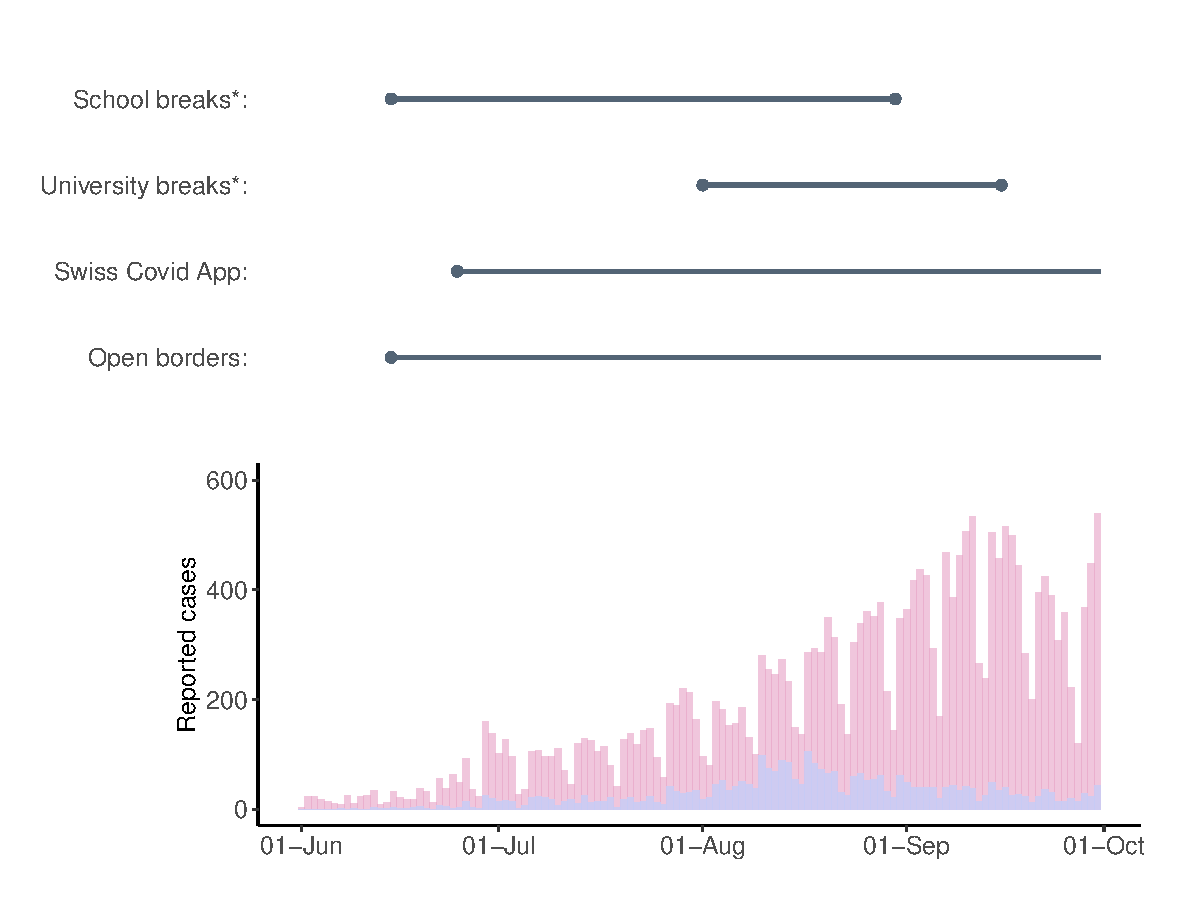
\includegraphics[scale=0.5]{regulation_cases_reported_2021-03-05.pdf}
\caption{Reported cases and major events: y-axis reported cases; x-axis time of interest; pink bars show all reported cases per day and violet bars show only cases with most likely place of infection abroad. *Official break of universities (might change for different subjects) and cantons have different school holiday, here we took earliest and latest holiday day. More details on quarantine measures  \href{https://www.fedlex.admin.ch/eli/cc/2021/61/de}{here}}.
\end{figure}
\begin{multicols}{2}

\end{multicols}
\begin{figure}[h]
\centering
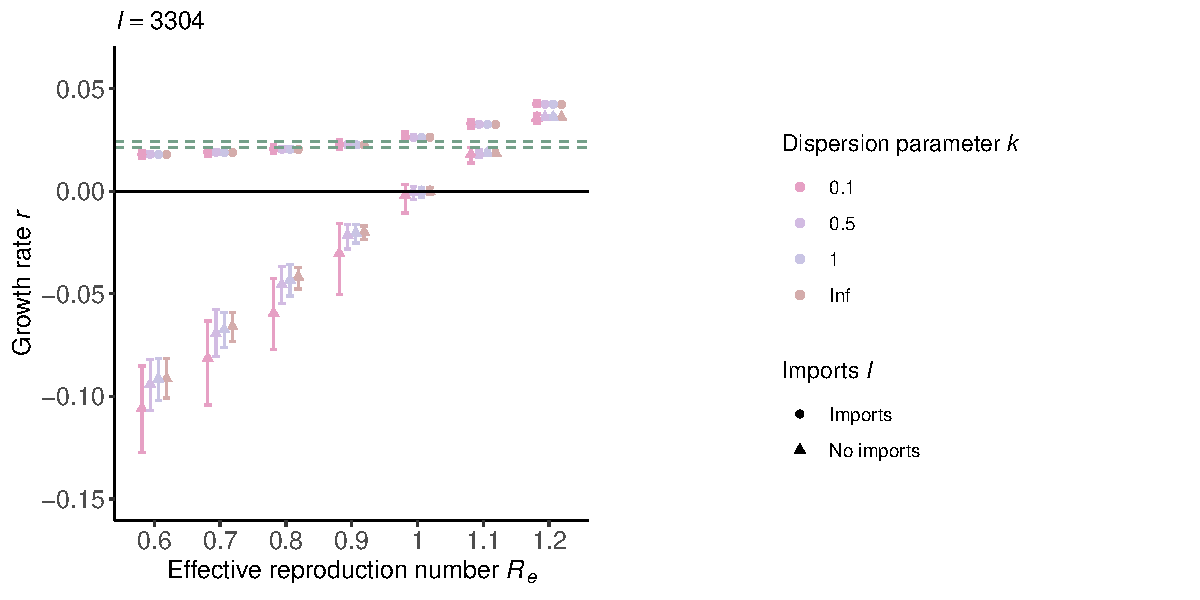
\includegraphics[scale=0.5]{growth_r_imports_infect_reported_2021-02-24.pdf}
\caption{Impact of imports on the epidemic growth rate: y-axis the epidemic growth rate; x-axis different $\mathcal{R}_e$ values; intervals show the inter-quantile range (IQR). Abbreviations: k, dispersion parameter; I, number of imports.}
\end{figure}
\begin{multicols}{2}

\end{multicols}
\begin{figure}[h]
\centering
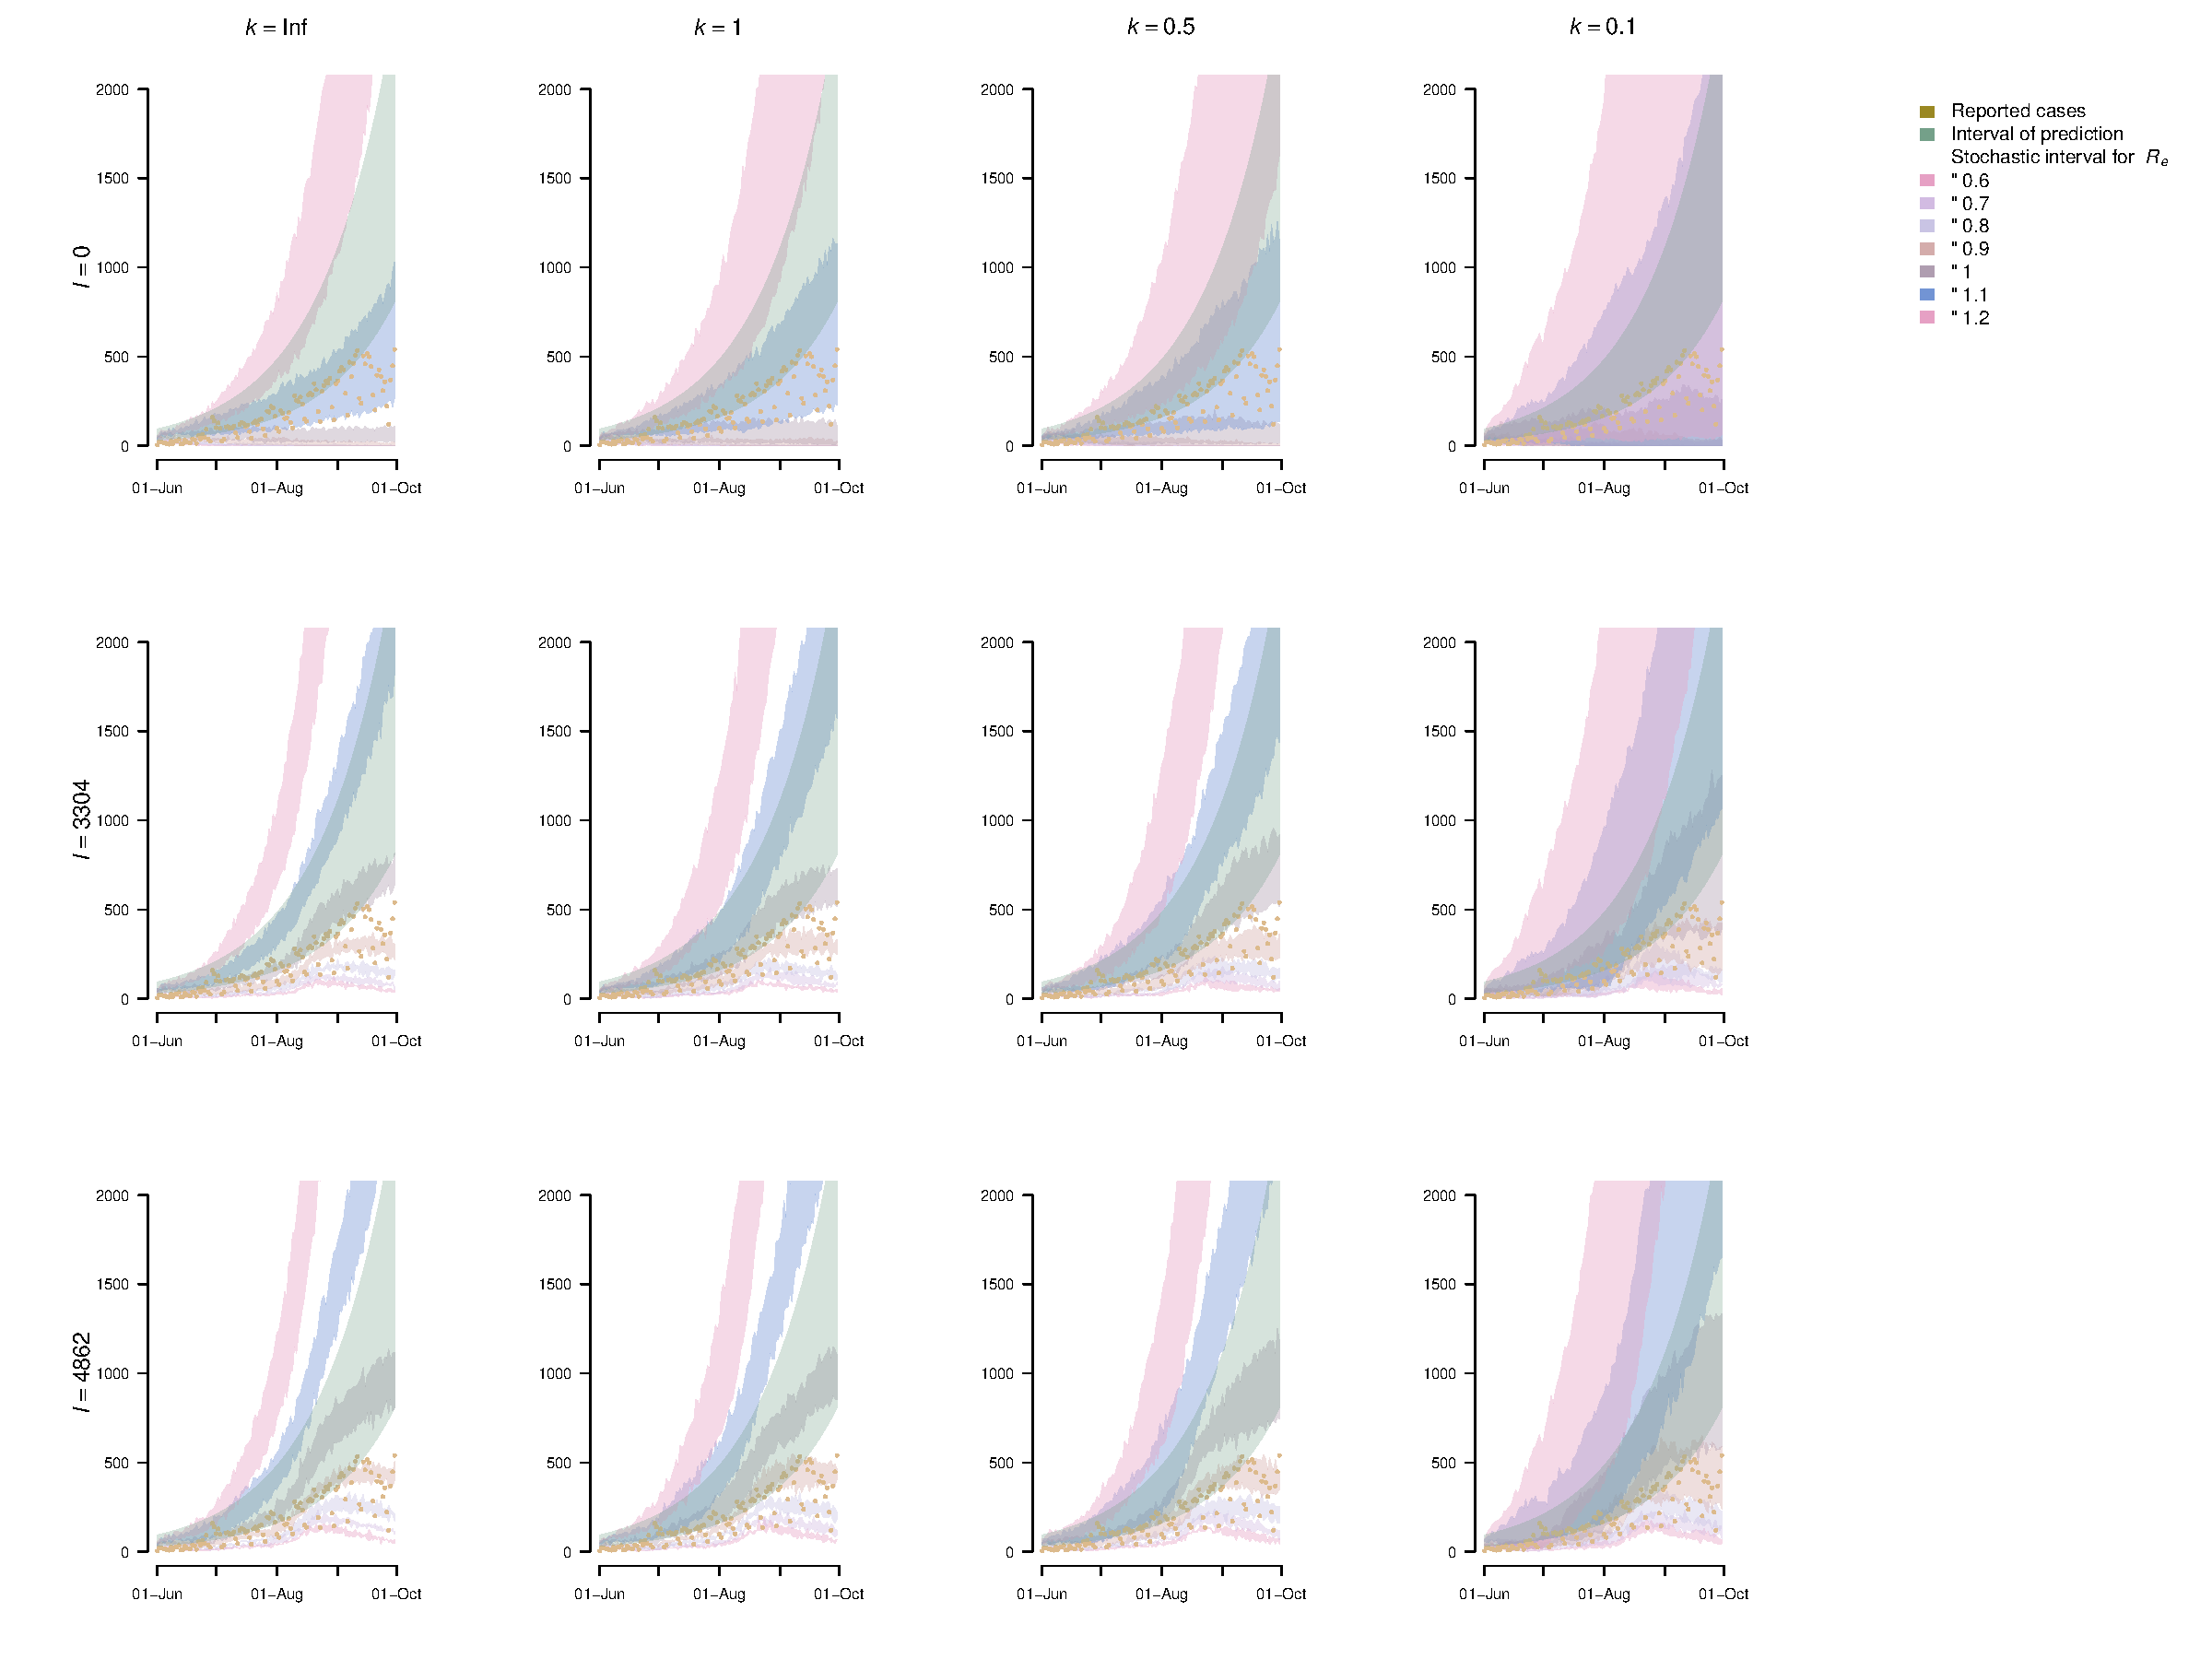
\includegraphics[scale=0.4]{sim3_cases_d_imports_infect_2021-02-24.pdf}
\caption{Impact of imports on the cases per day: y-axis cases per day; x-axis time of interest. Yellow dots show the reported cases per day and green area shows the predicted cases per day. Abbreviations: $k$, dispersion parameter; $I$, number of imports.}
\end{figure}

\begin{multicols}{2}

\section{Discussion}
The SARS-CoV-2 epidemic grew from a few dozen confirmed cases per day in early June 2020 to several hundred by the end of September 2020. 
Switzerland is a relatively small country with a few million inhabitants, but due to its location (and its wealth) there is a high potential for travel to have a huge impact on the epidemic.
Therefore, the intrinsic high probability of extinction - due to the small number of cases in early June - may have been offset by travel.
We estimated a $\mathcal{R}_e$ slightly above 1 for the time of interest. So, the $\mathcal{R}_e$ was around the critical value of 1, where small changes have a huge effect on the epidemic. 
Our stochastic simulations showed that the national epidemic had a $\mathcal{R}_e$ below one, i.e. a value below the critical threshold. 
Travel-associated cases and their further transmission was a leading force that led to several hundred cases per day by the end of September 2020. 
Without any travel-associated cases, regardless of the dispersion parameter $k$, only an $\mathcal{R}_e$ above 1 could explain the observed Swiss epidemic. 
In our analysis, we only accounted for travel-associated case that were successfully detected and thus stoped their transmission chain or for travel-associated case that infected further in the same way as cases that were infected in Switzerland.
\textcolor{red}{Need to include sth on age differences.}


\textcolor{red}{Nevertheless, our method has limitations that need to be addressed. We did not account for different behaviour in different groups. With our model we could only estimate a broad spectrum for the effect of travel-associated cases}

Quantifying the role of imports on the national dynamics of SARS-CoV-2 epidemics requires further investigation. 
In Switzerland, travel-associated case might have had a considerable impact on the national dynamics and could explain the growth of the SARS-CoV-2 epidemic during summer 2020. 
Our results underline the importance of improved surveillance for international travellers in order to better control the spread of SARS-CoV-2.

\section{Acknowledgement}
We thank the FOPH.

\section{Author contributions}
MLR, EBH, JR, and CLR conceived the study and contributed to the analysis of the results. 
MLR performed the analysis and wrote the first draft of the manuscript. 
%NH gave important inputs for the analysis and interpretation. 
All authors read and approved the final manuscript.

\section{Funding}
European Union’s Horizon 2020 research and innovation programme - project EpiPose (No 101003688). Swiss National Science Foundation (grant 196046)

\section{Reference}

\bibliography{su2020_cov2.bib}
\bibliographystyle{vancouver}

\end{multicols}

\clearpage
\section{Supplementary}
\begin{suppfigure}[h]
\centering
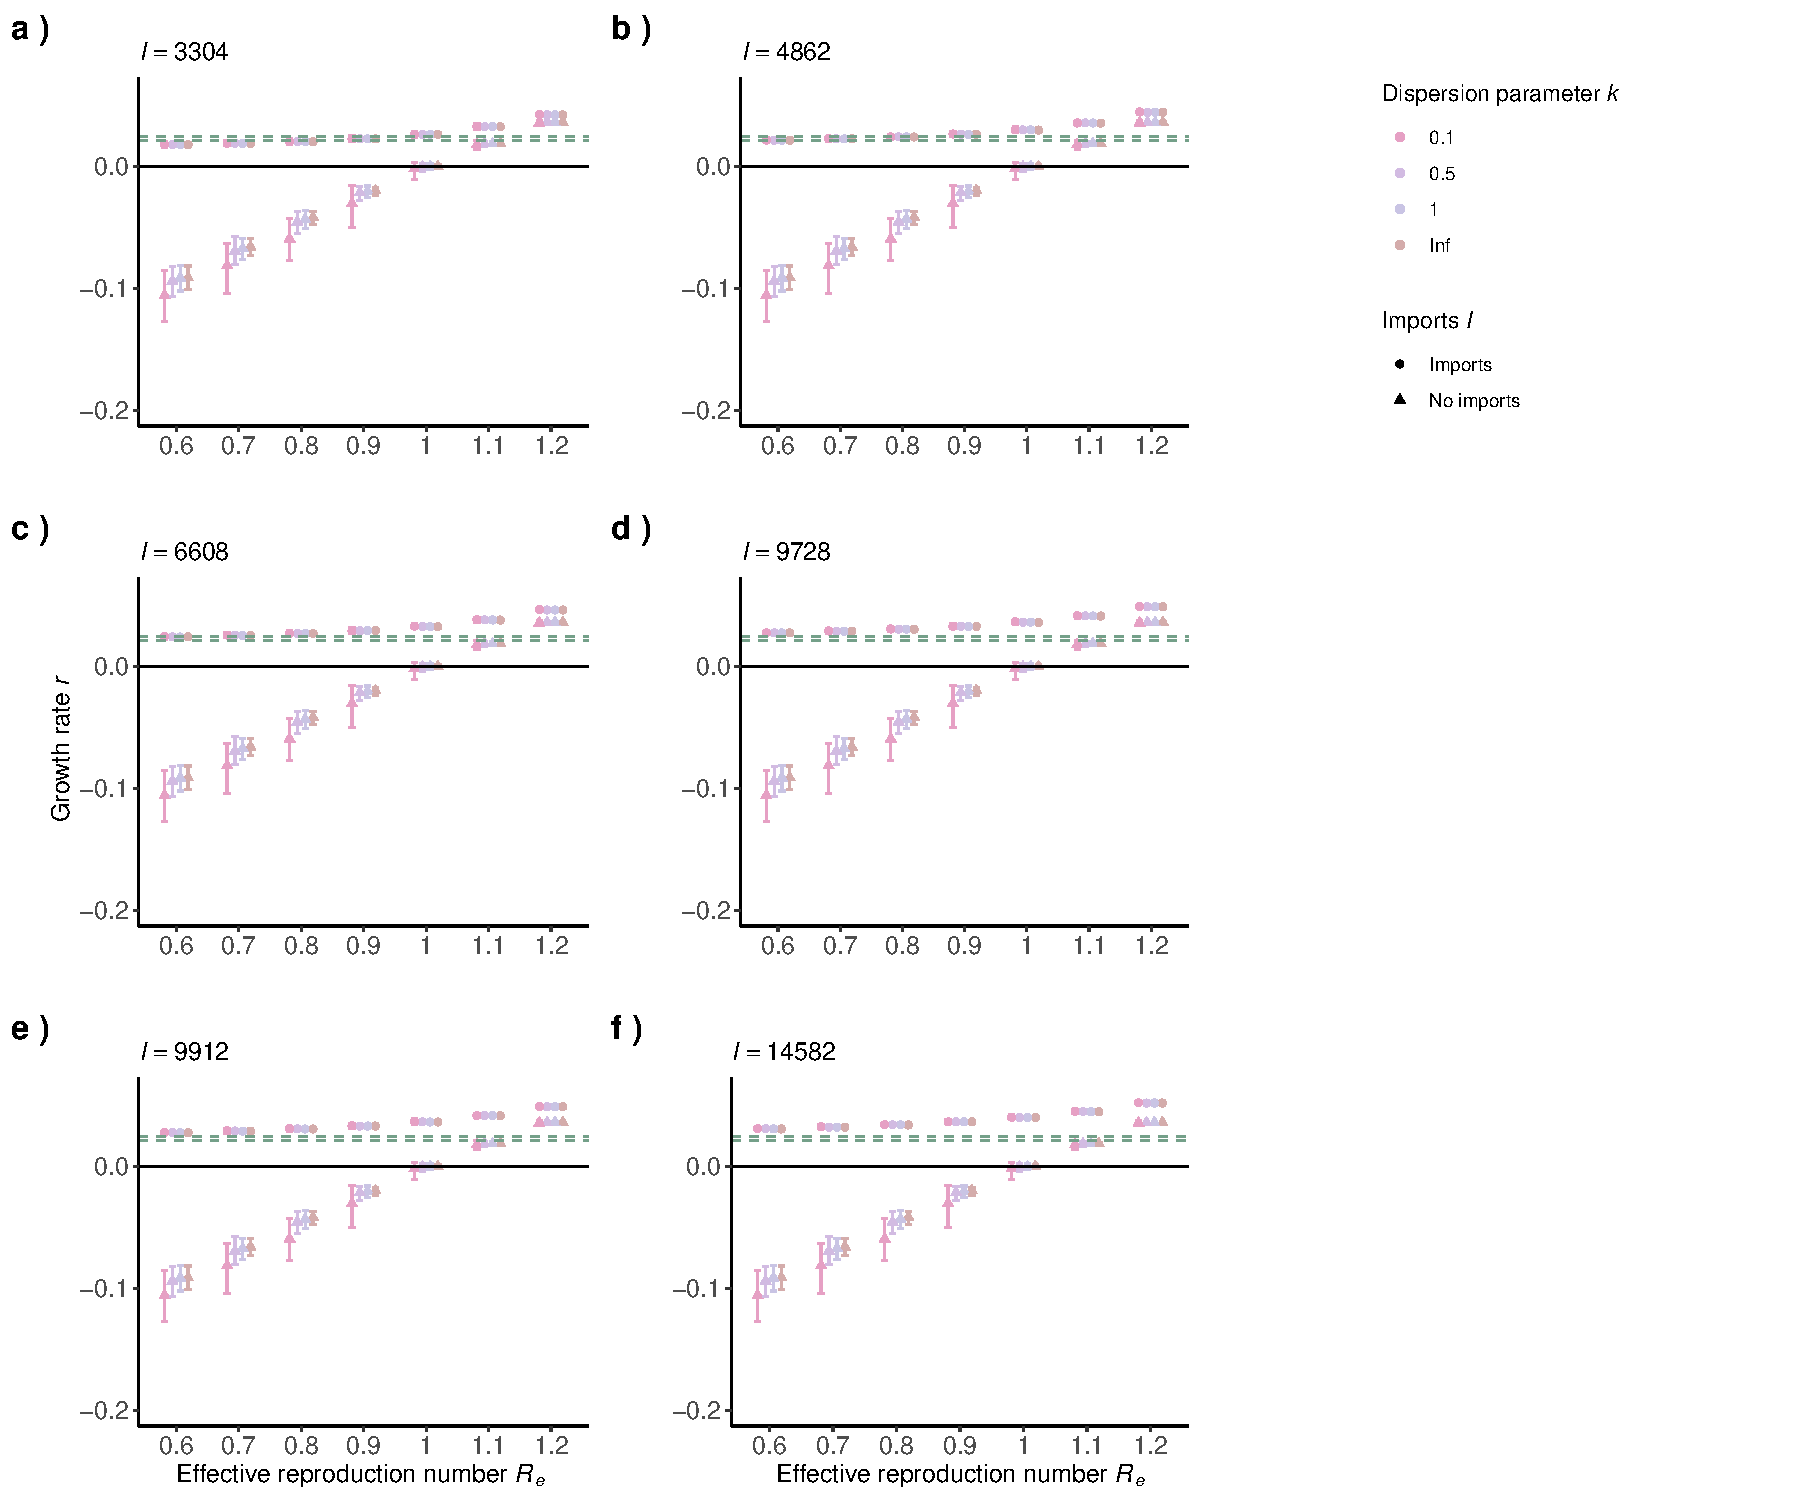
\includegraphics[scale=0.5]{growth_r_imports_infect_2021-02-24.pdf}
\caption{Impact of travel-associated cases \emph{I} that infect further on the epidemic growth rate: y-axis the epidemic growth rate; x-axis different $\mathcal{R}_e$ values; intervals show the inter-quantile range (IQR). a) reported travel-associated cases. b) reported imports multiplied by following $1+ \frac{\Sigma ~of ~cases ~with ~unknown ~origin }{\Sigma ~of ~all ~confirmed ~cases}$. c) $a)$ multiplied with 2. d) $b)$ multiplied with 2. e,f) $a)$ and $b)$ multiplied with 3, respectively. Abbreviations: k, dispersion parameter; I, number of travel associated cases.}
\end{suppfigure}
\clearpage
\begin{suppfigure}[h]
\centering
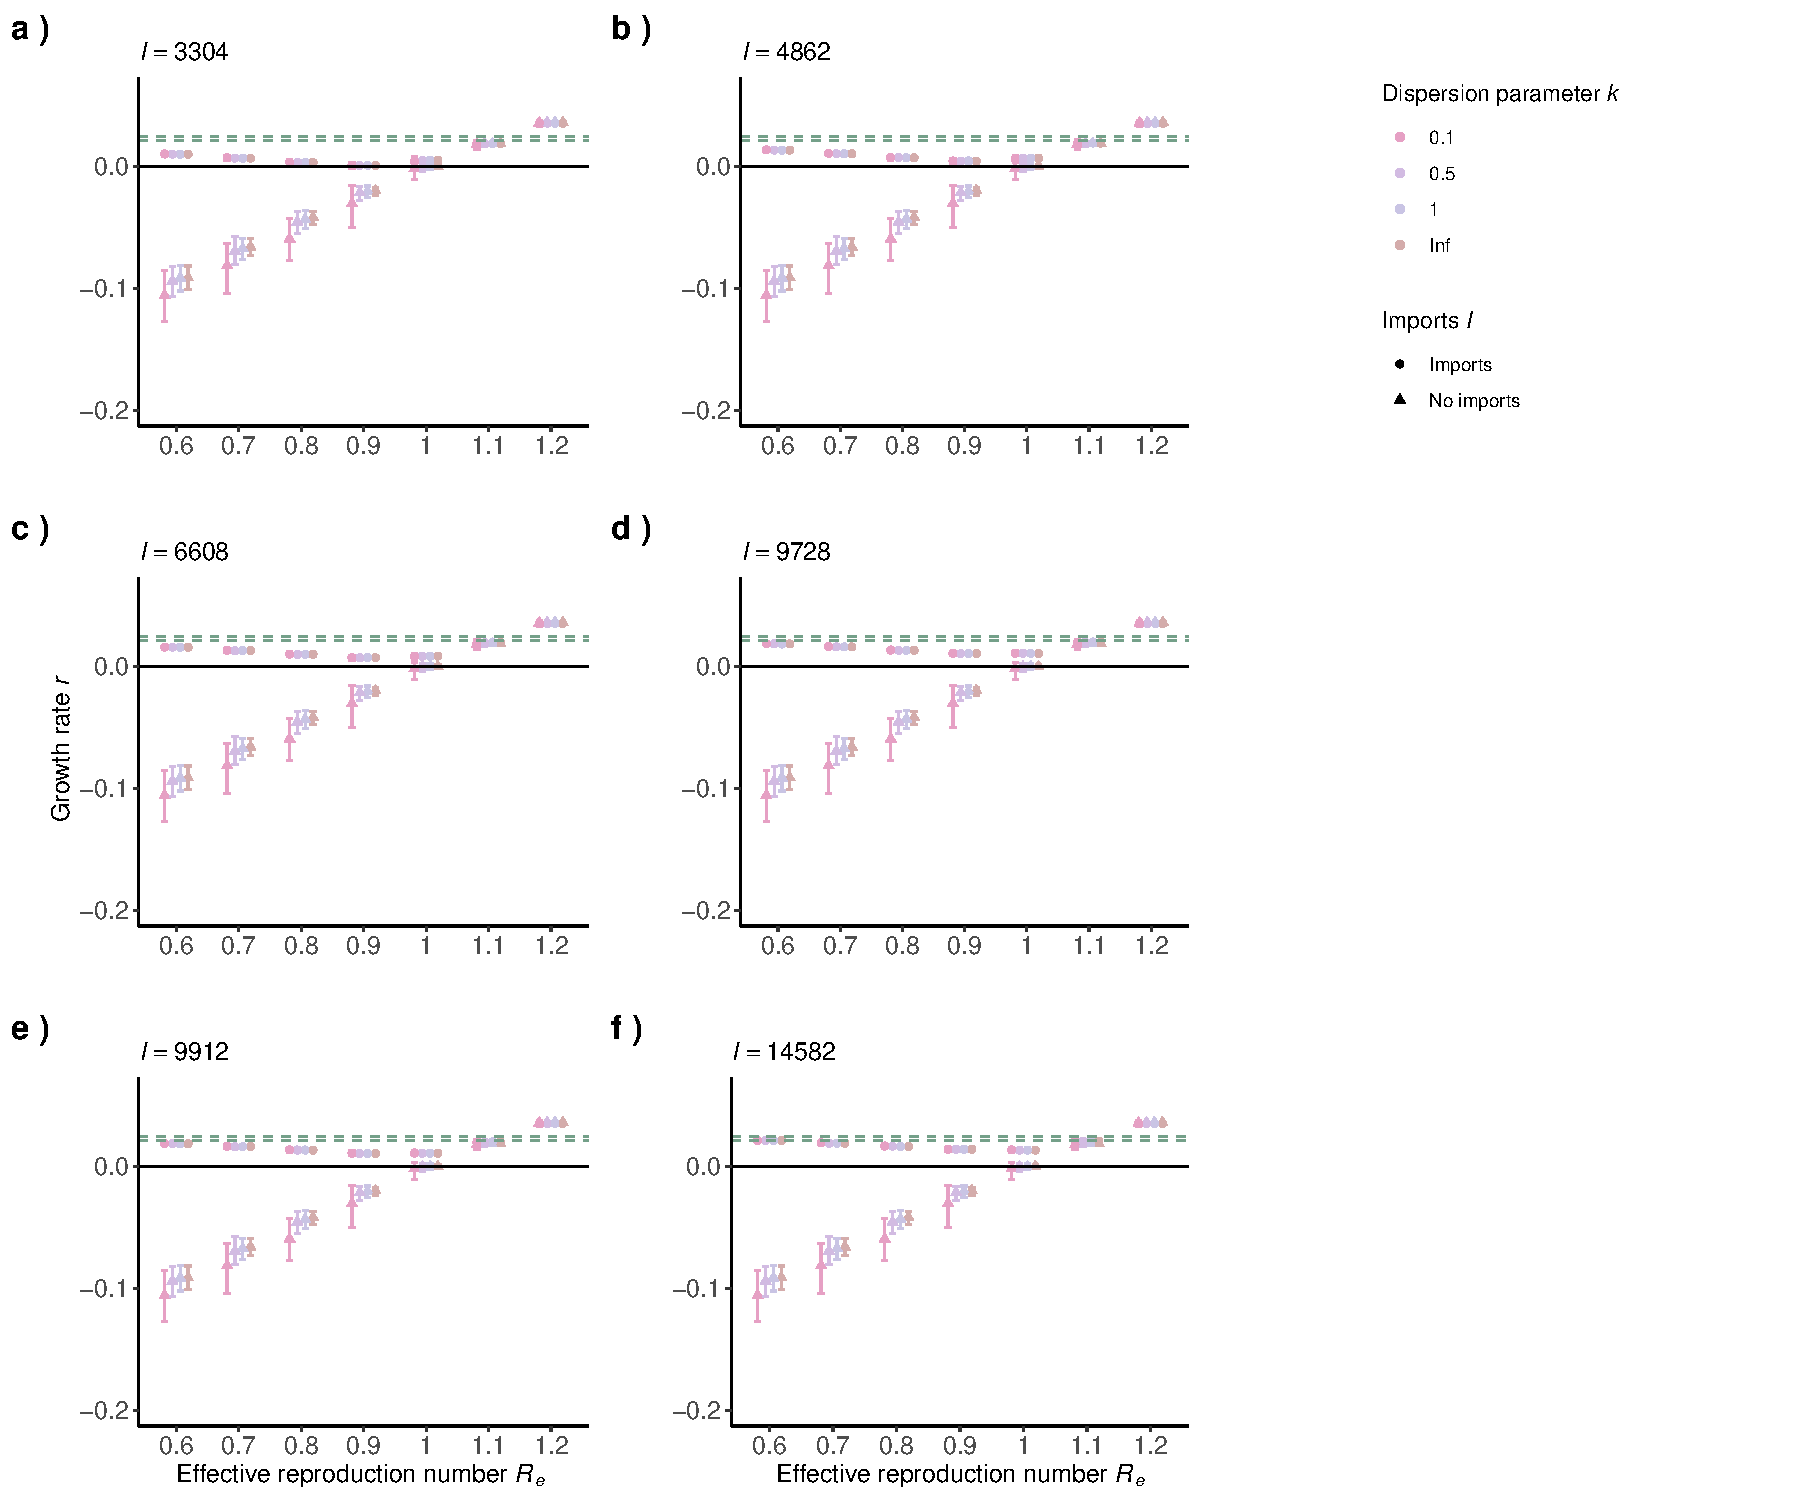
\includegraphics[scale=0.5]{growth_r_imports_2021-02-24.pdf}
\caption{Impact of travel associated cases \emph{I} that do not infect further on the epidemic growth rate: y-axis shows the epidemic growth rate; x-axis different $\mathcal{R}_e$ values; intervals show the inter-quantile range (IQR). a) reported travel associated cases. b) reported imports multiplied by following $1+ \frac{\Sigma ~of ~cases ~with ~unknown ~origin }{\Sigma ~of ~all ~confirmed ~cases}$. c) $a)$ multiplied with 2. d) $b)$ multiplied with 2. e,f) $a)$ and $b)$ multiplied with 3, respectively. Abbreviations: k, dispersion parameter; I, number of travel associated cases.}
\end{suppfigure}
\clearpage
\begin{suppfigure}[h]
\centering
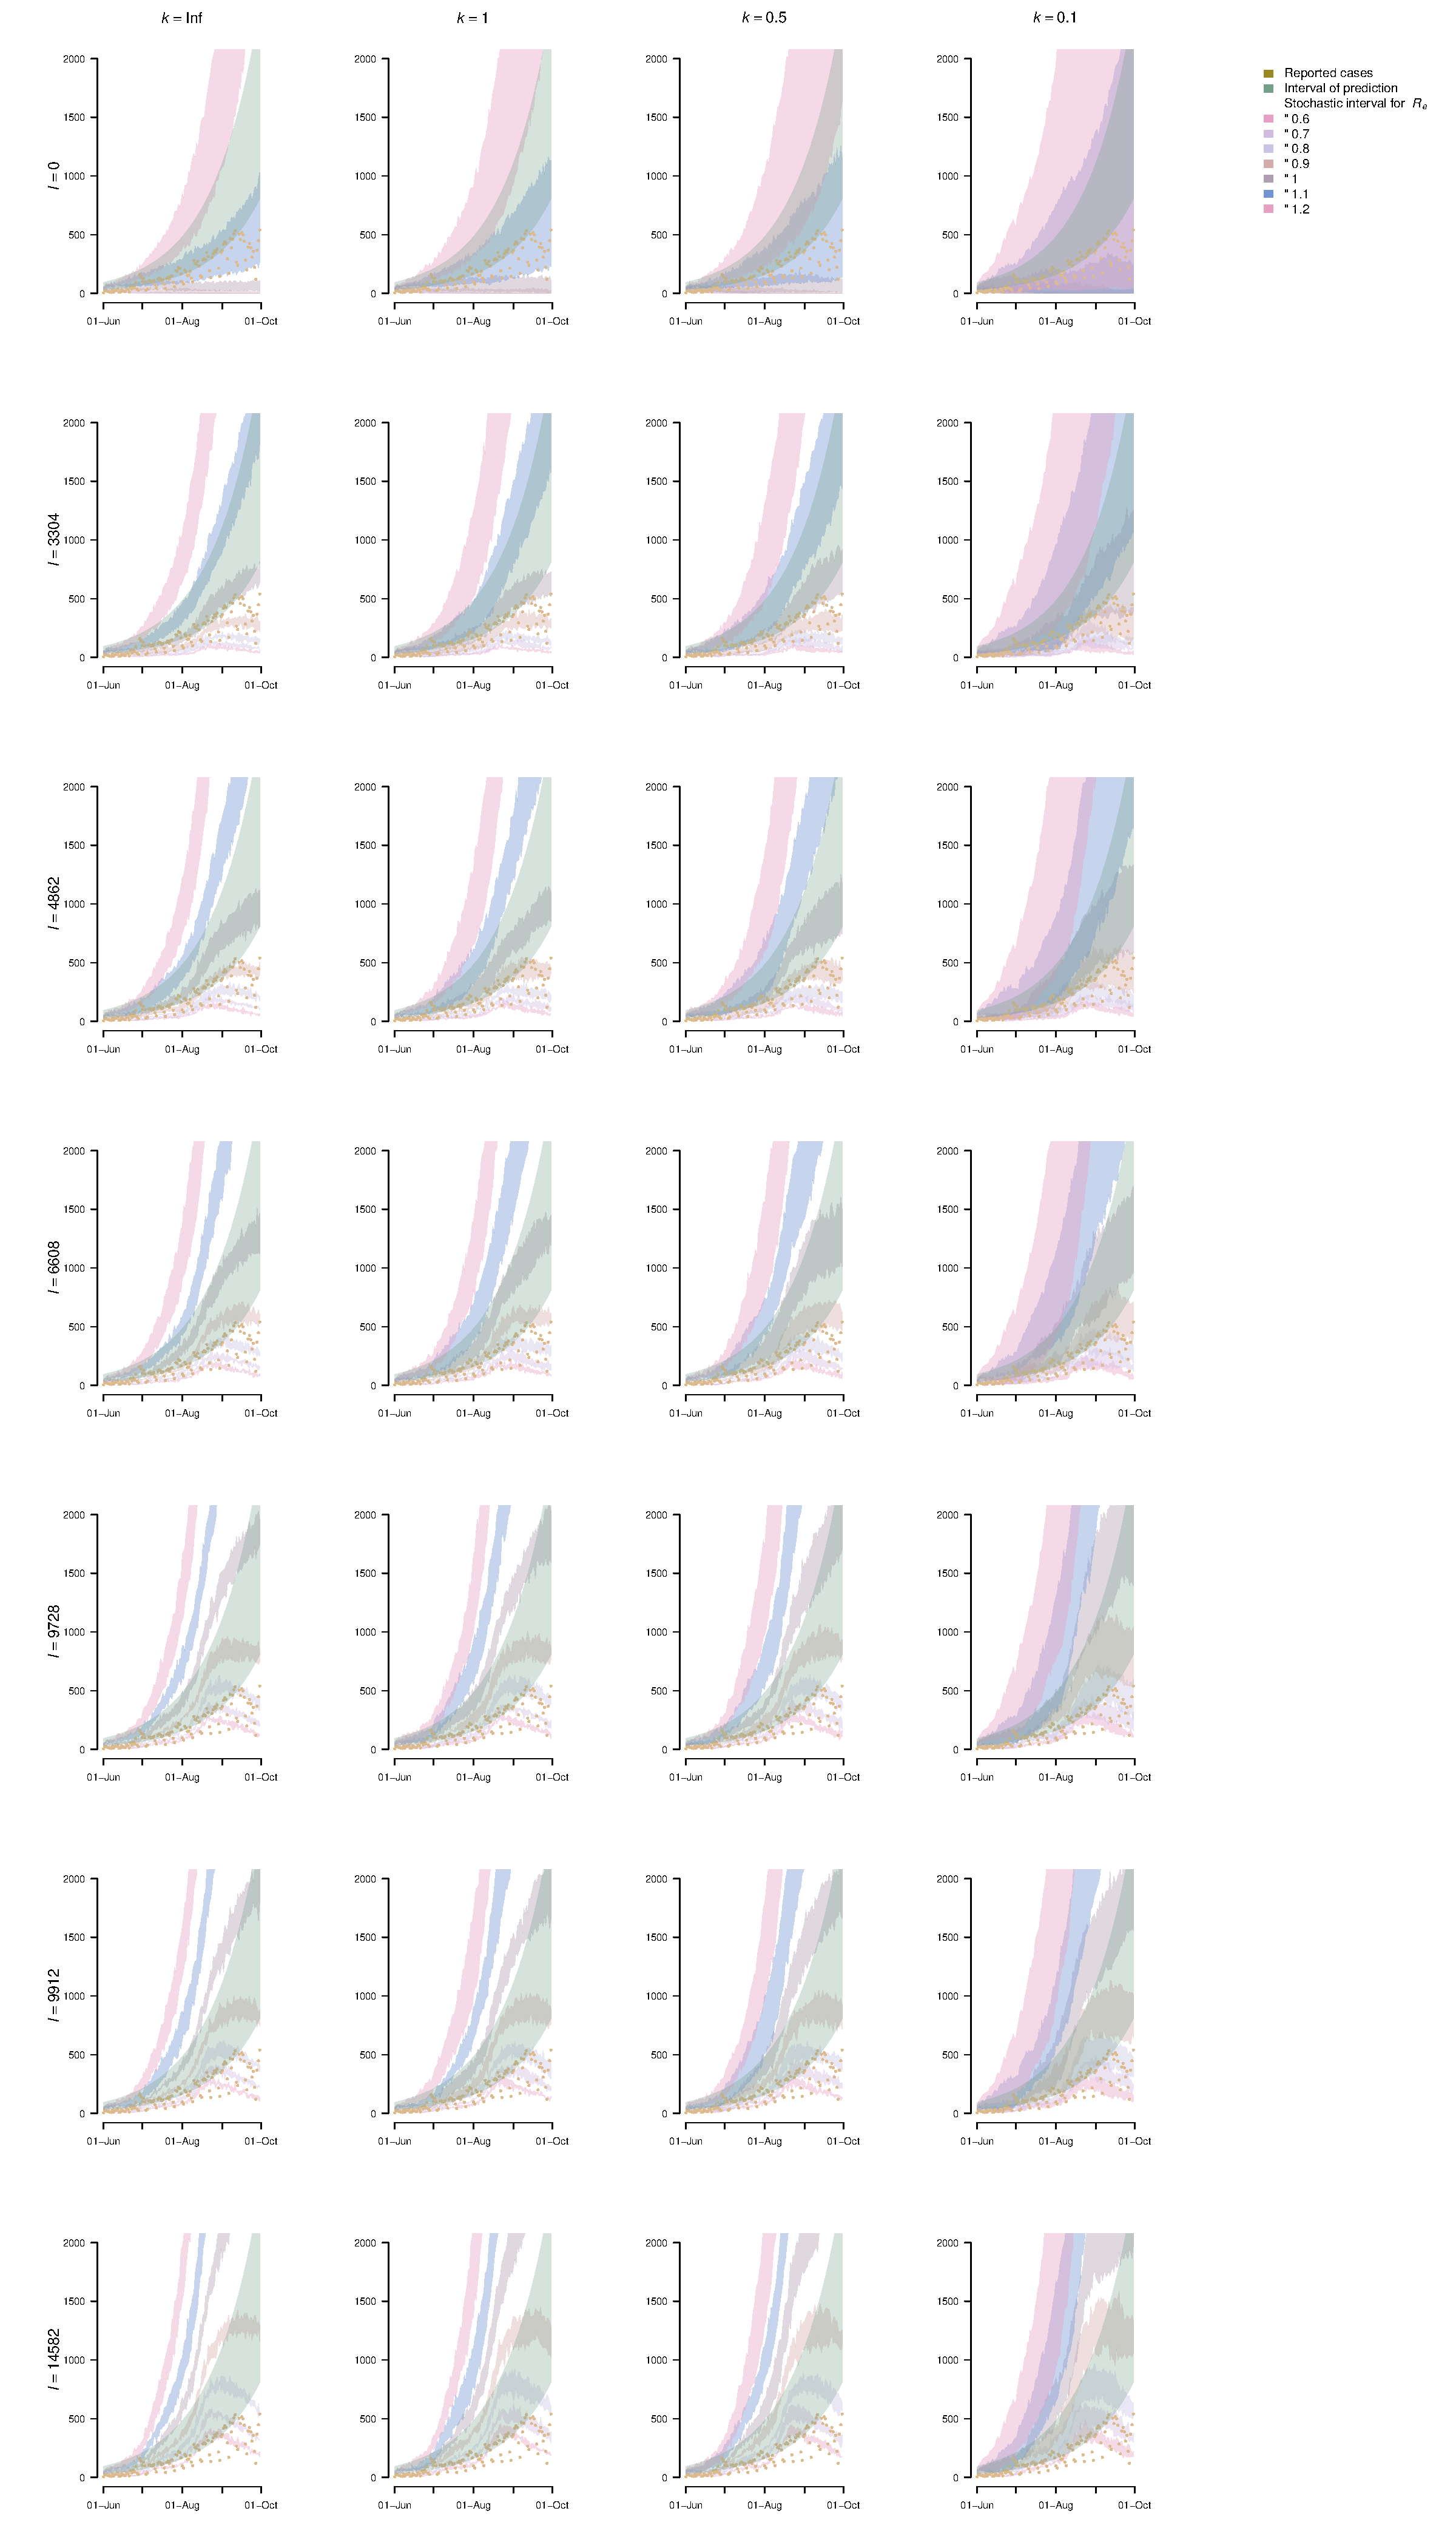
\includegraphics[scale=0.3]{sim_cases_d_imports_infect_2021-02-24.pdf}
\caption{Impact of travel-associated cases on the cases per day that infected further: y-axis cases per day; x-axis the time of interest. Different number of travel-associated cases \emph{I} were added to a stochastic branching model whereby these \emph{I} could transmit further: \emph{I} was zero, reported \emph{I}, reported \emph{I} multiplied by $1+ \frac{\Sigma ~of ~cases ~with ~unknown ~origin }{\Sigma ~of ~all ~confirmed ~cases}$, and these multiplied with 2 and 3, respectively. Yellow dots show the reported cases per day and green area shows the predicted cases per day. Abbreviations: k, dispersion parameter; I, number of travel associated cases.}
\end{suppfigure}
\clearpage
\begin{suppfigure}[h]
\centering
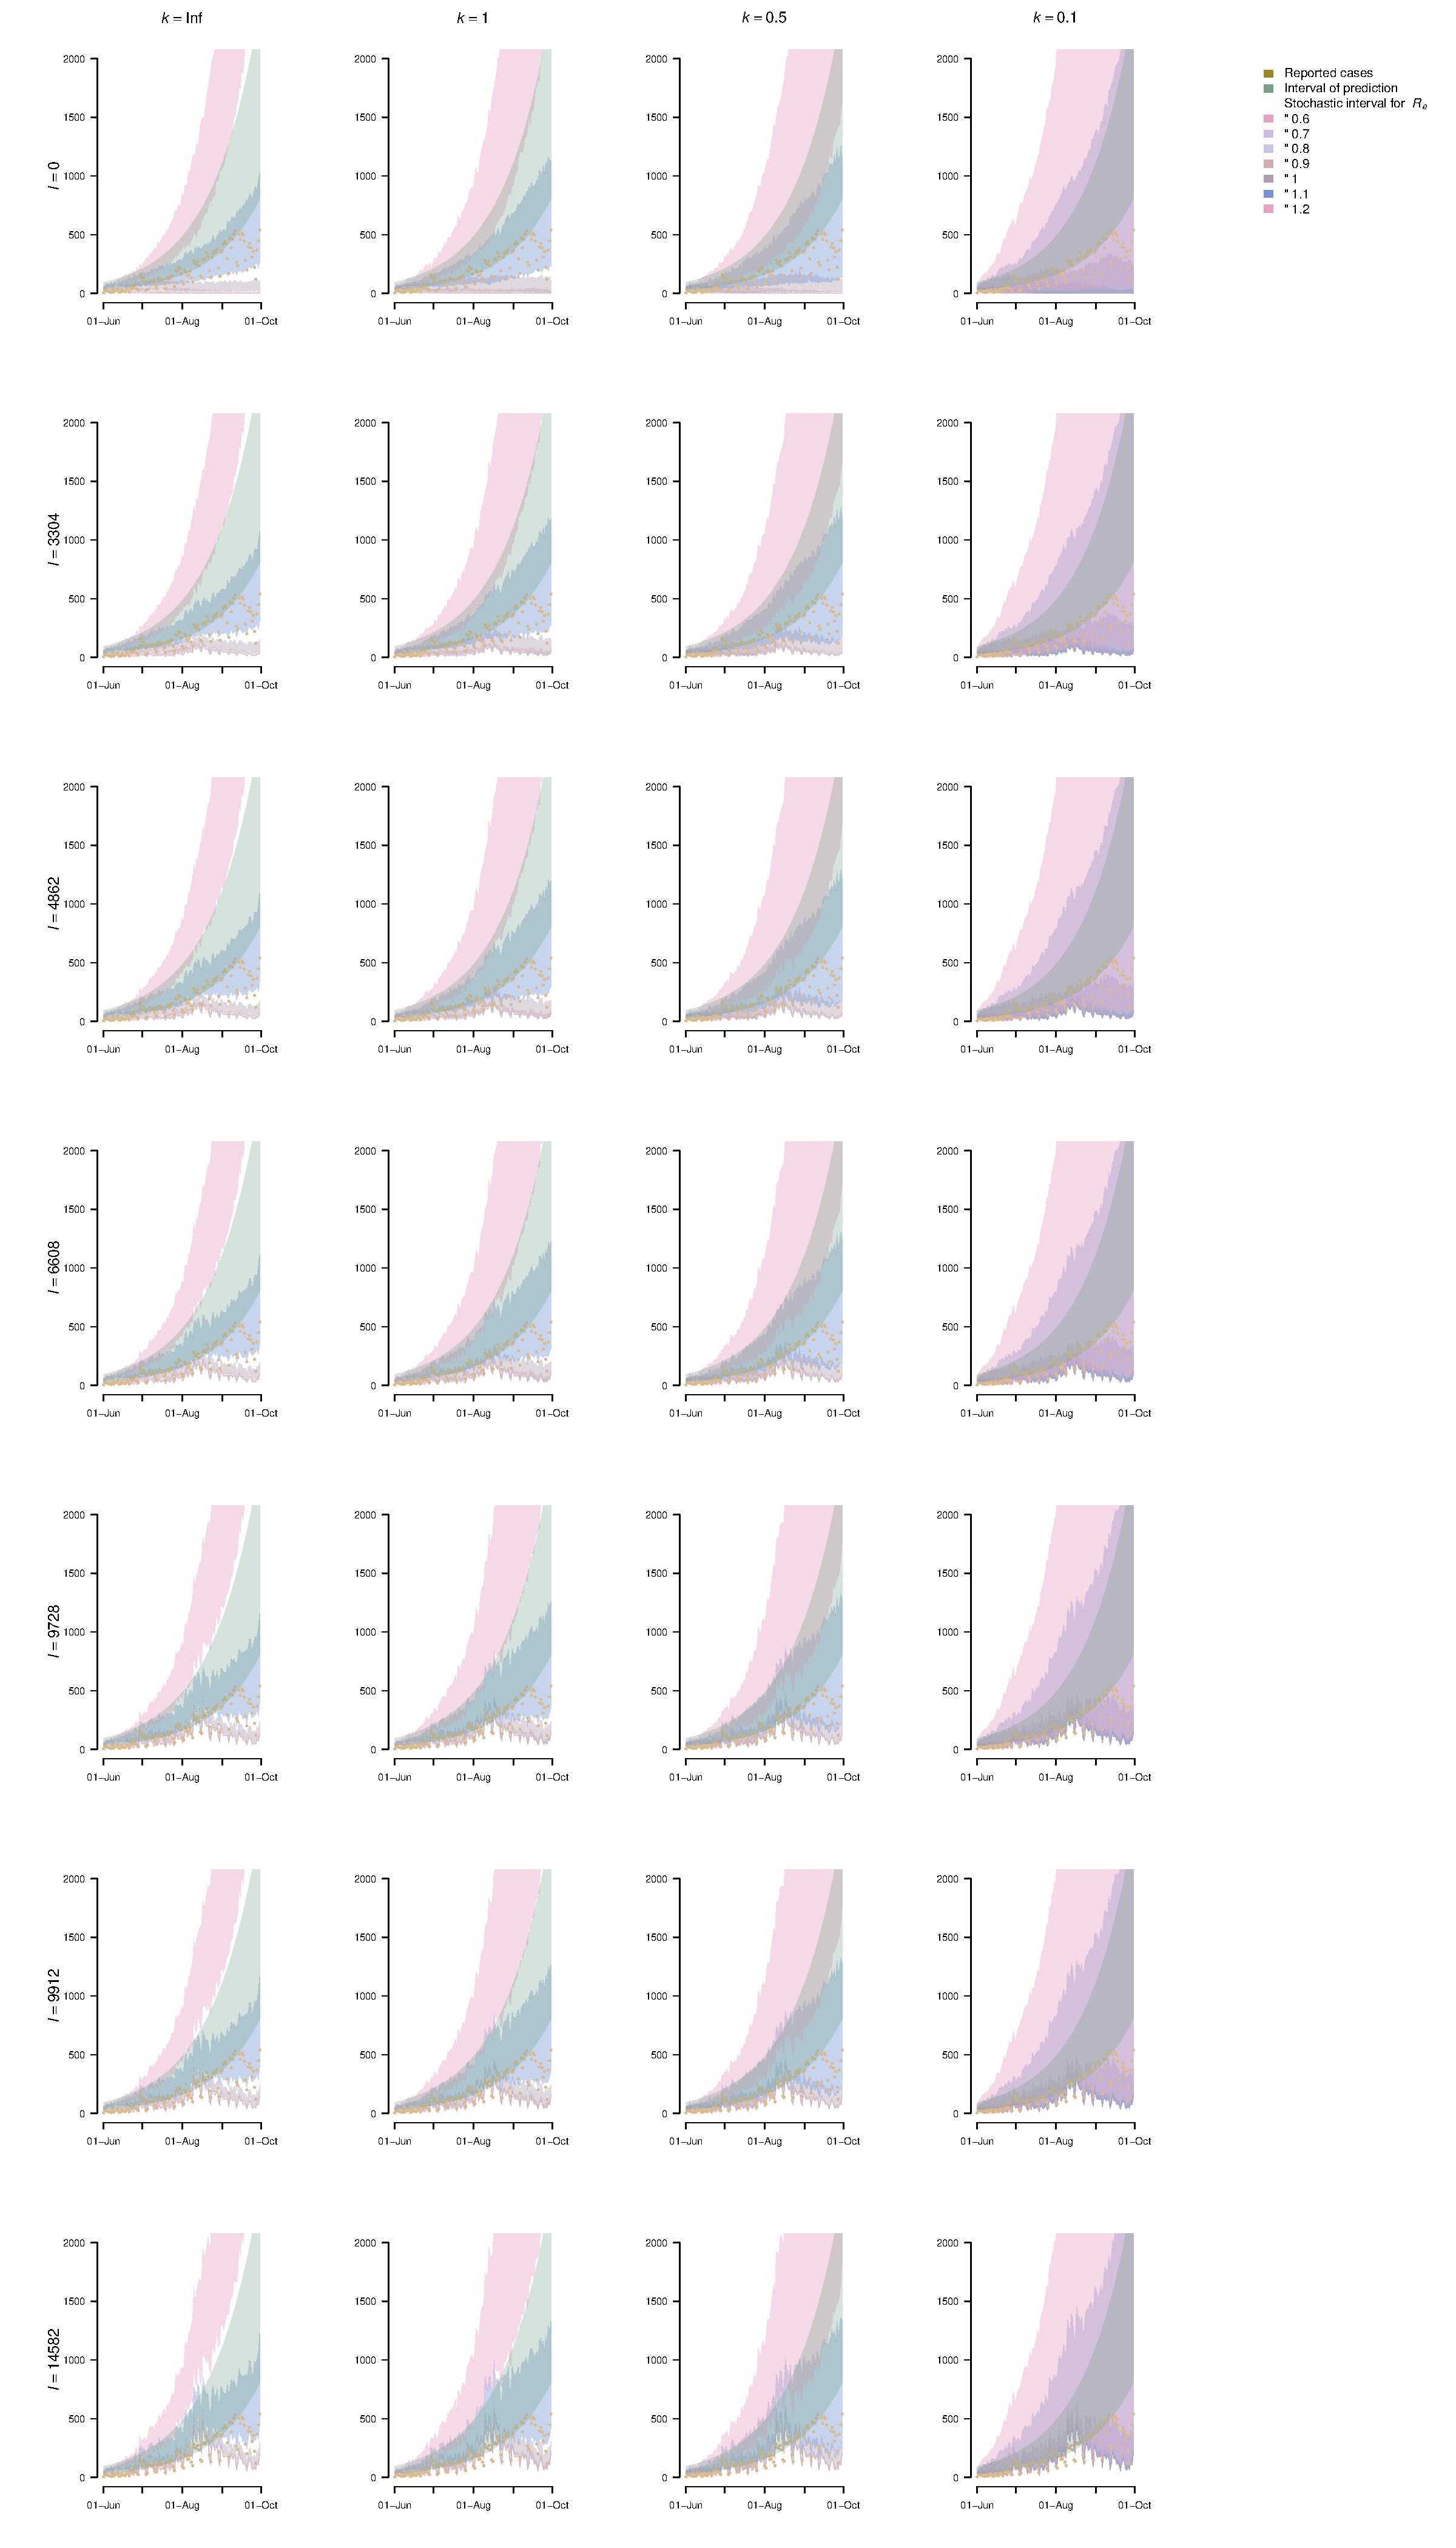
\includegraphics[scale=0.3]{sim_cases_d_imports_2021-02-24.pdf}
\caption{Impact of travel-associated cases on the cases per day that did not infect further: y-axis cases per day; x-axis the time of interest. Different number of travel-associated cases \emph{I} were added to a stochastic branching model whereby these \emph{I} could transmit further: \emph{I} was zero, reported \emph{I}, reported \emph{I} multiplied by $1+ \frac{\Sigma ~of ~cases ~with ~unknown ~origin }{\Sigma ~of ~all ~confirmed ~cases}$, and these multiplied with 2 and 3, respectively. Yellow dots show the reported cases per day and green area shows the predicted cases per day. Abbreviations: k, dispersion parameter; I, number of travel associated cases.}
\end{suppfigure}
\clearpage
\begin{suppfigure}[h]
\centering
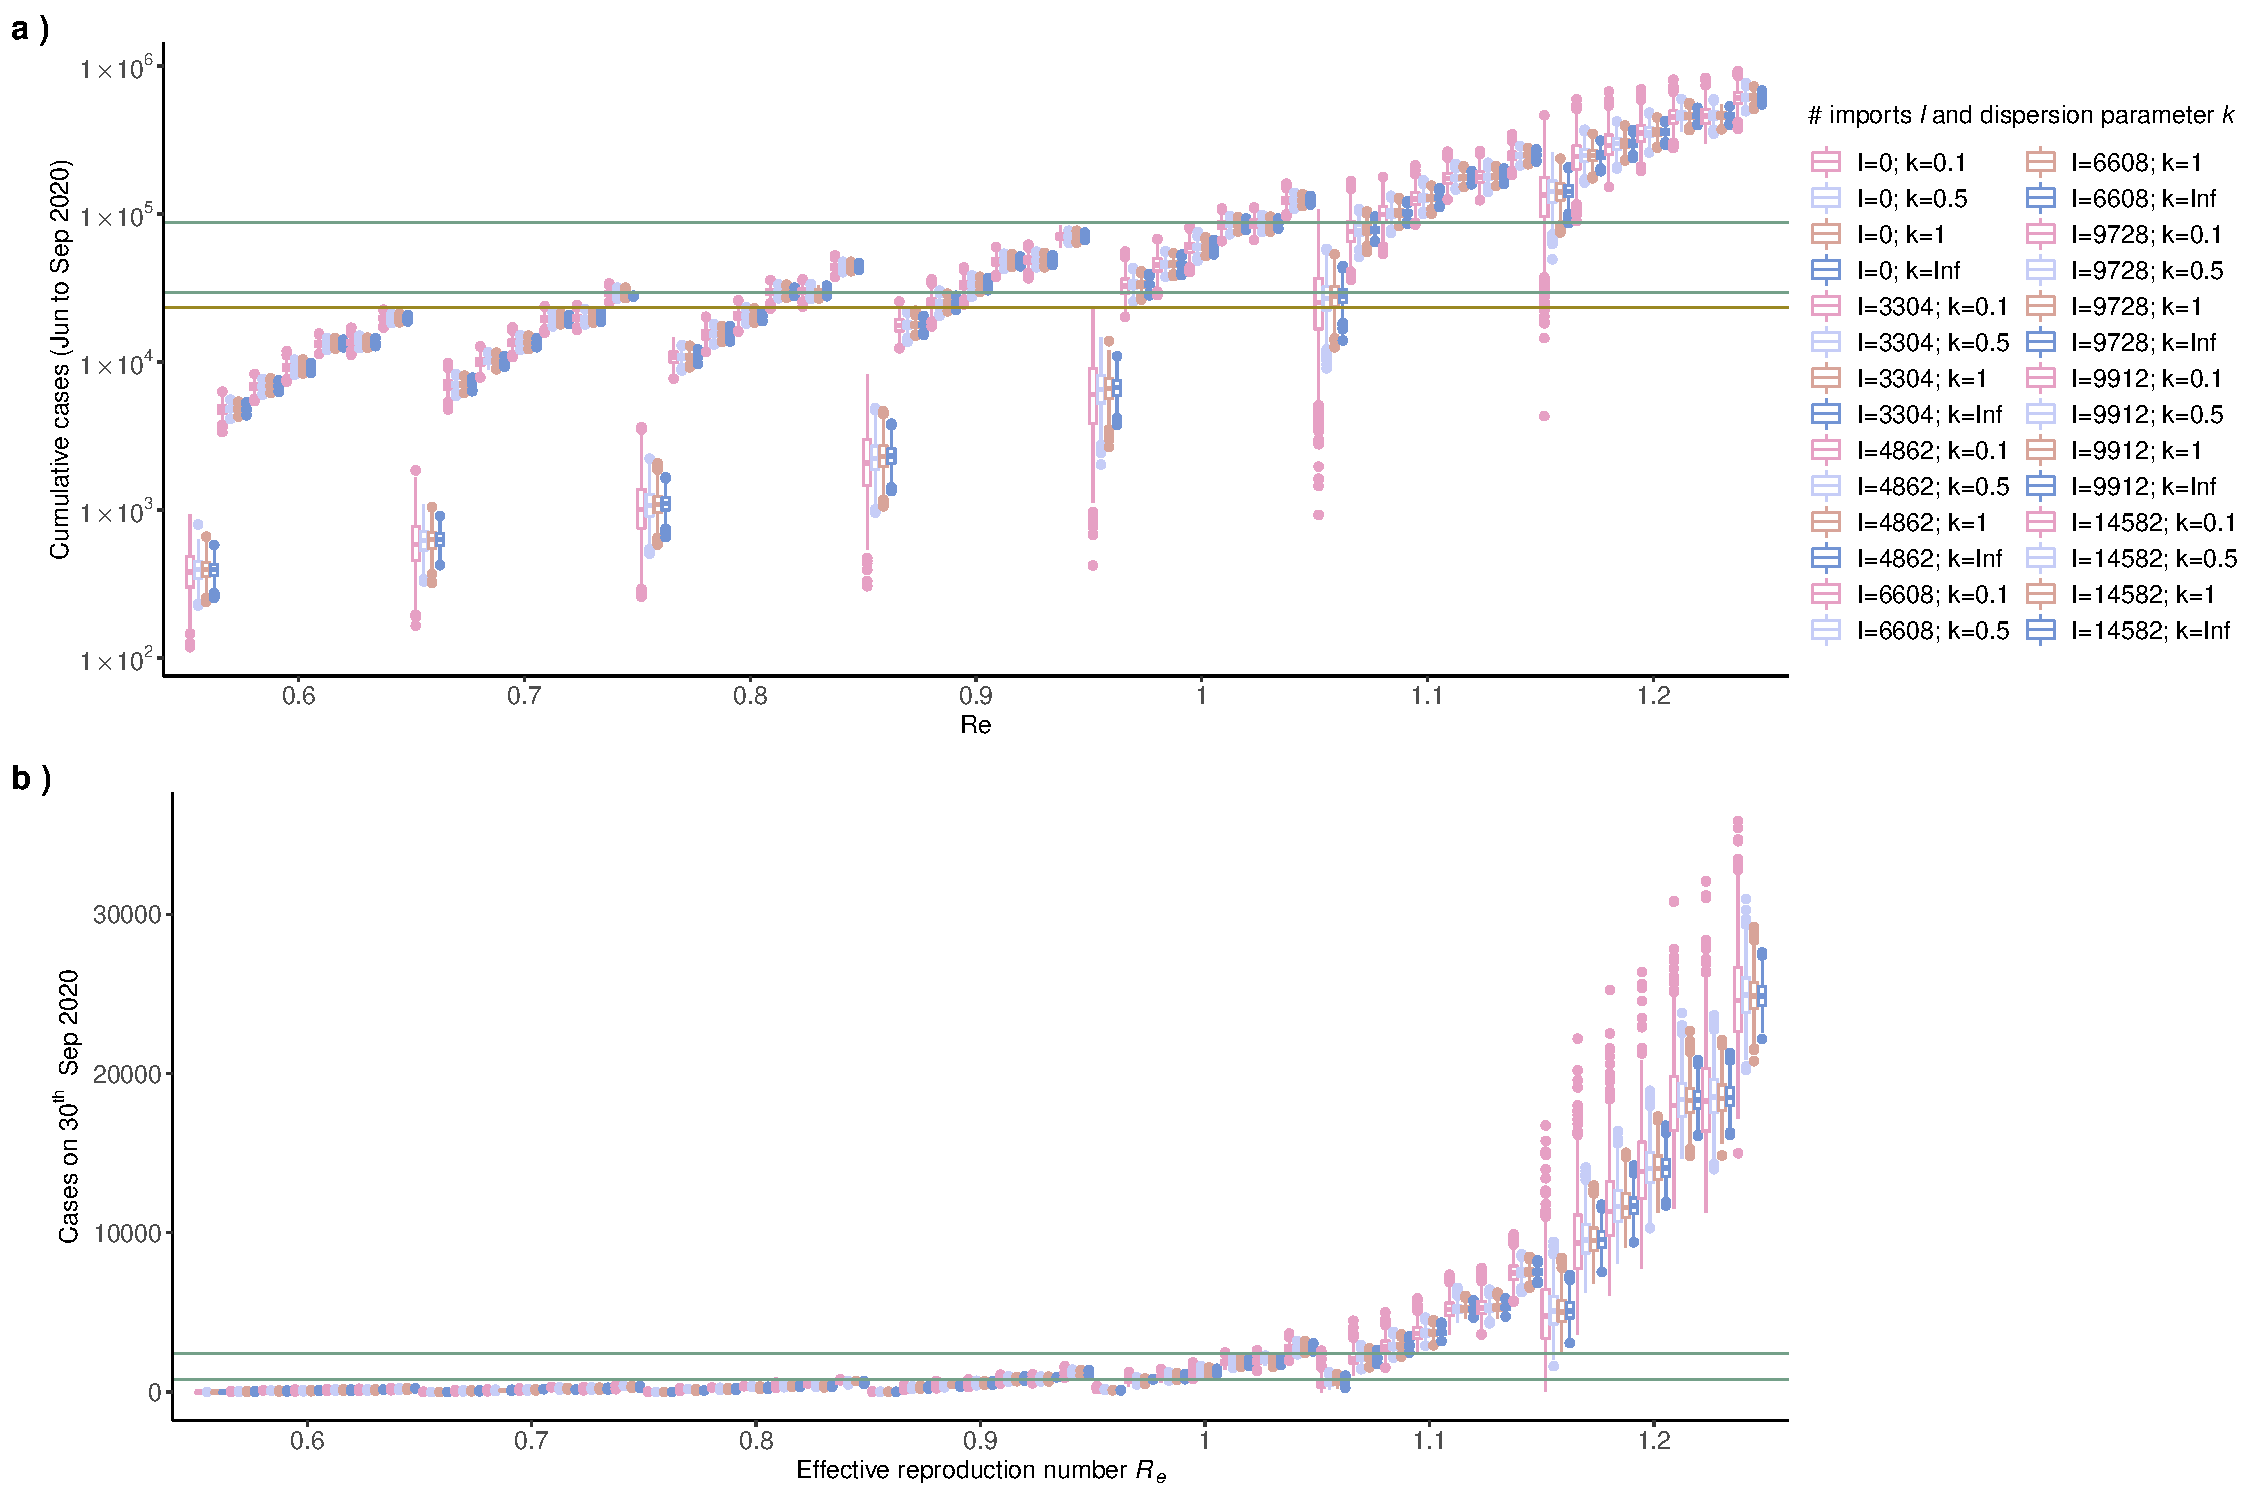
\includegraphics[scale=0.4]{size_scenarios_imports_infect_2021-02-24.pdf}
\caption{Cumulative cases and final number of cases regarding the different scenarios whereby travel-associated cases infected further.Yellow line shows the reported cases during $1^{st}$ of June to $30^{th}$ of September 2020. The area between the green lines shows the predicted cases during $1^{st}$ of June to $30^{th}$ of September 2020 and on the $30^{th}$ of September 2020. Abbreviations: k, dispersion parameter; I, number of travel associated cases.}
\end{suppfigure}
\clearpage
\begin{suppfigure}[h]
\centering
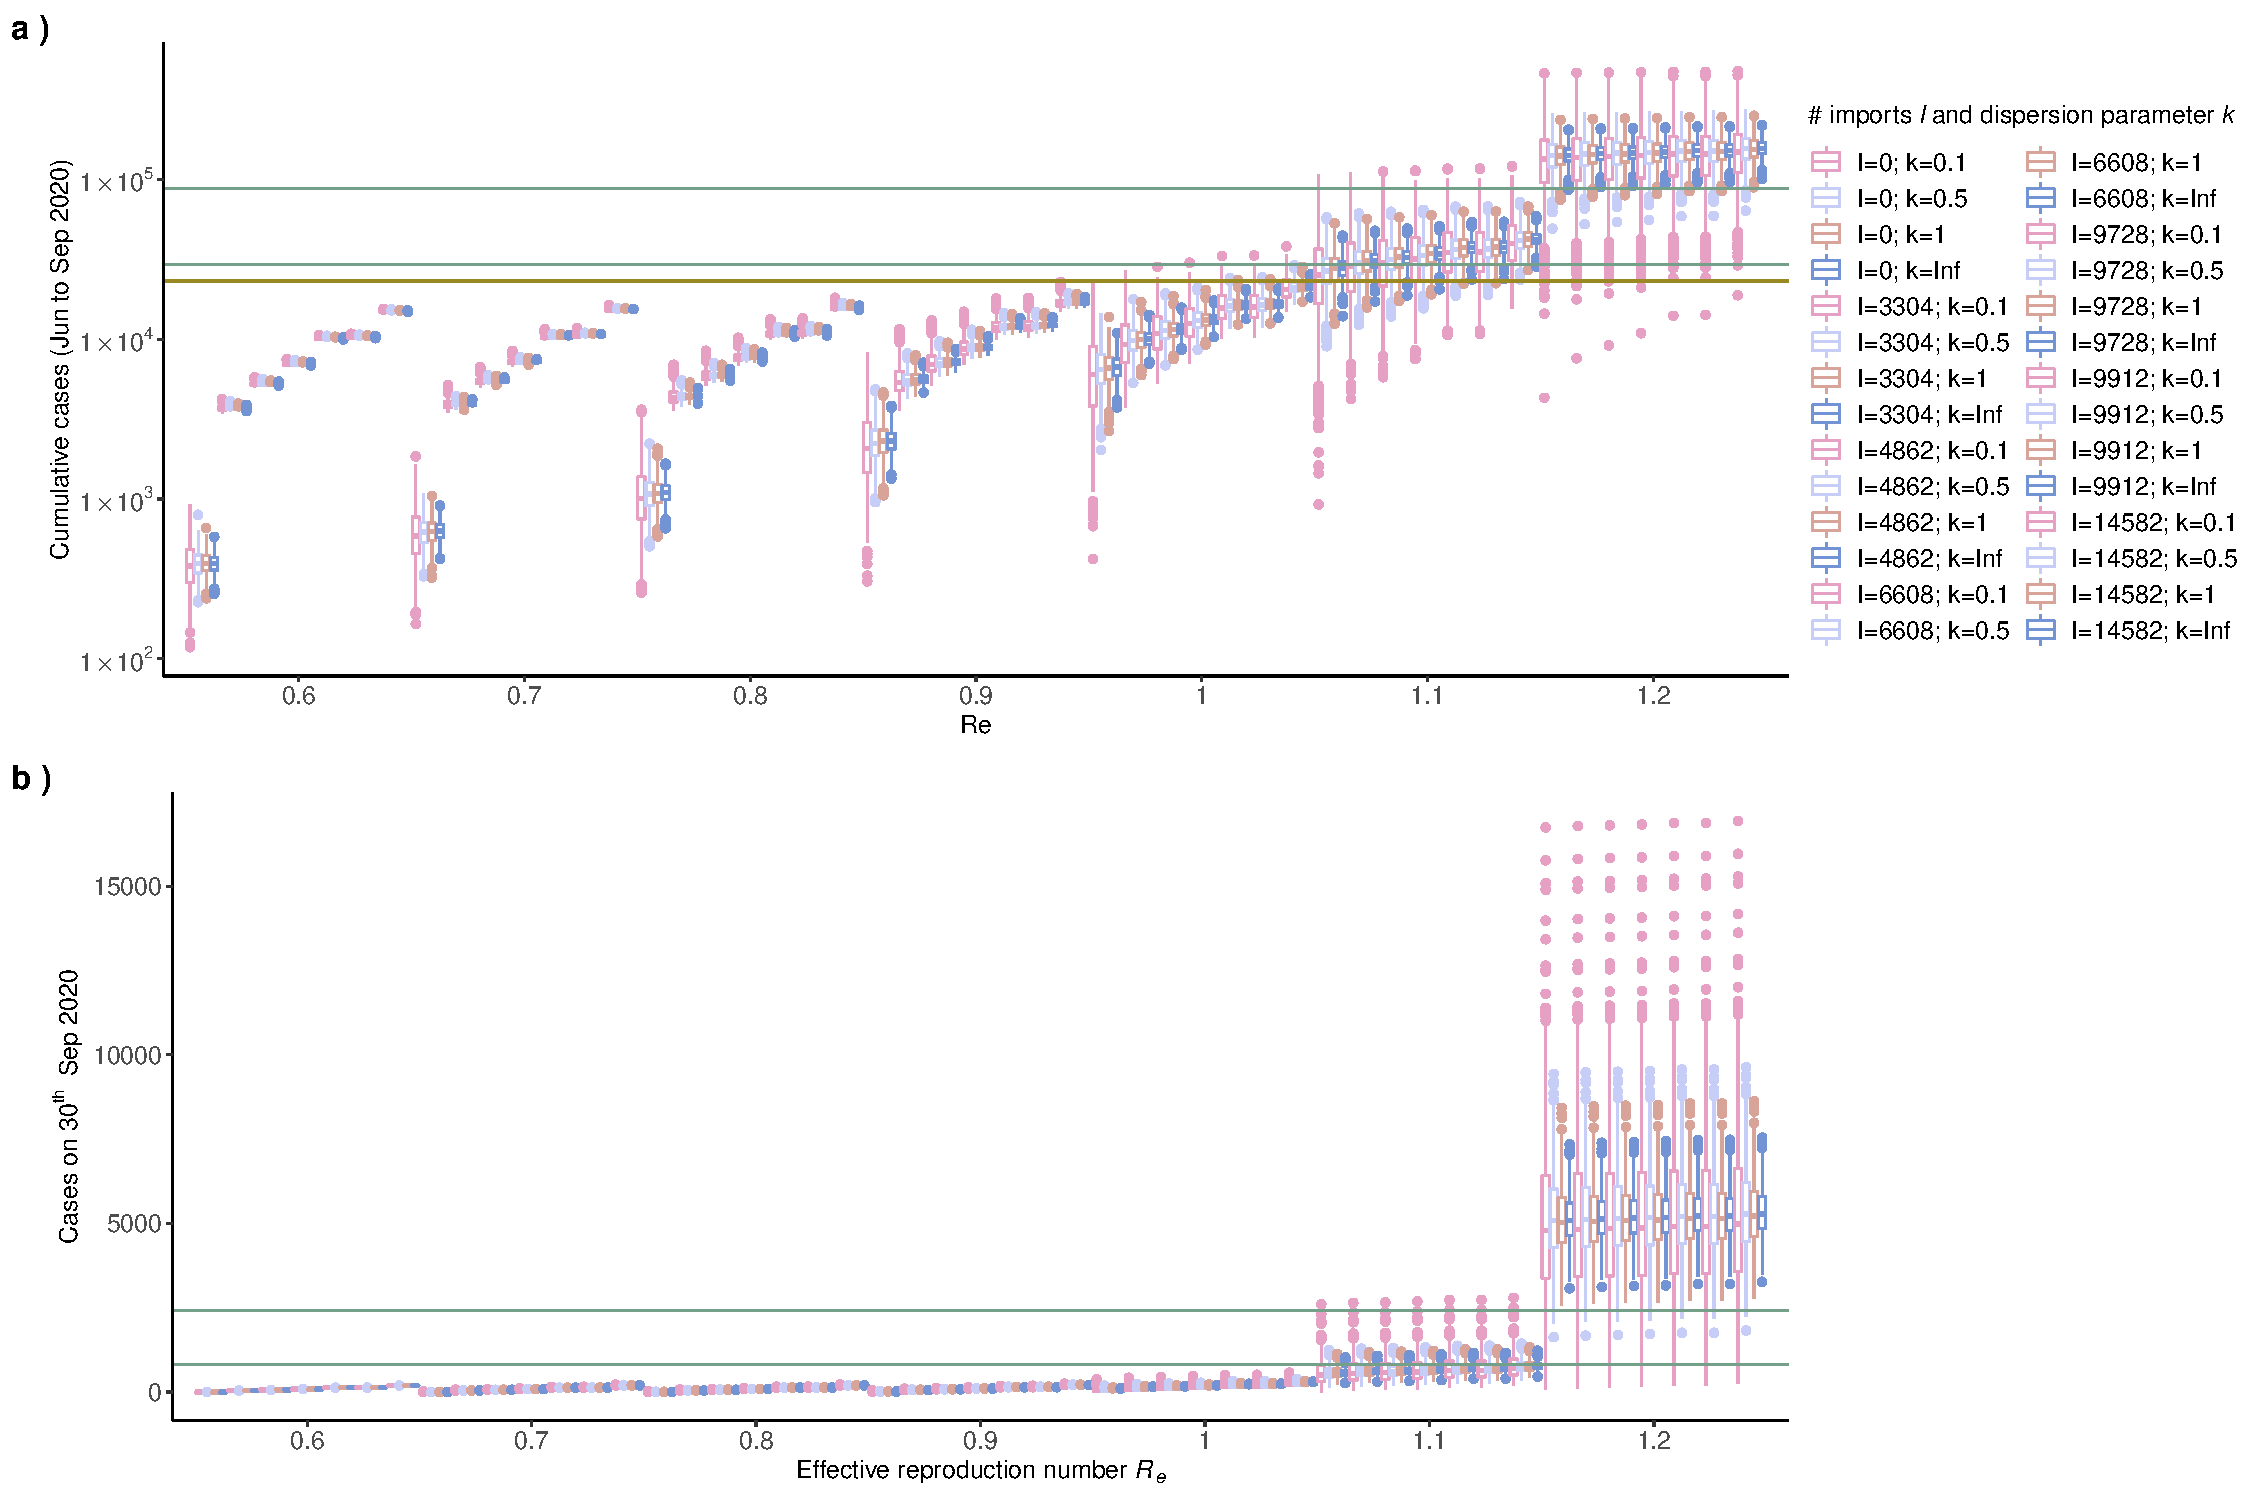
\includegraphics[scale=0.4]{size_scenarios_imports_2021-02-24.pdf}
\caption{Cumulative cases and final number of cases regarding the different scenarios whereby travel-associated cases did not infect further. Yellow line shows the reported cases during $1^{st}$ of June to $30^{th}$ of September 2020. The area between the green lines shows the predicted cases during $1^{st}$ of June to $30^{th}$ of September 2020 and on the $30^{th}$ of September 2020. Abbreviations: k, dispersion parameter; I, number of travel associated cases.}
\end{suppfigure}
\clearpage
\begin{suppfigure}[h]
\centering
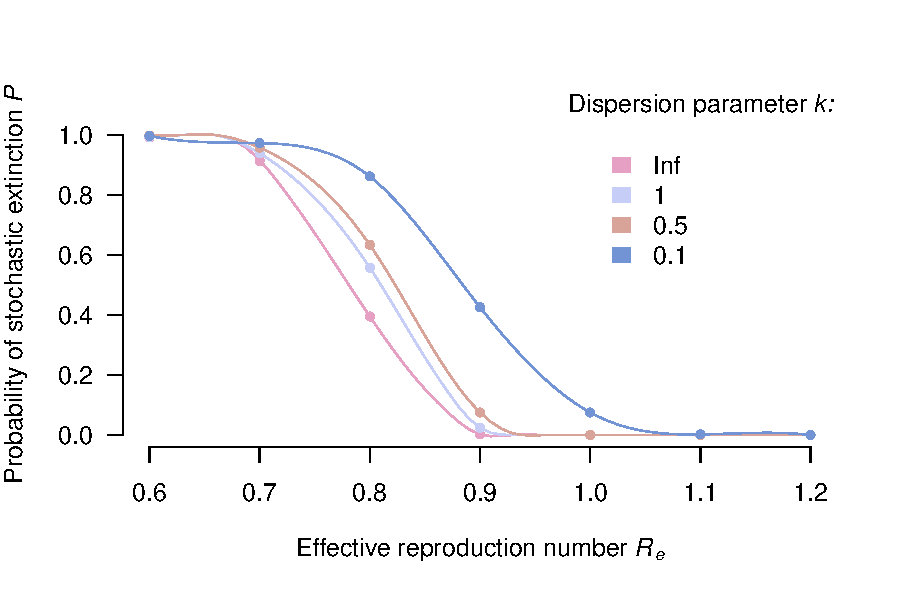
\includegraphics[scale=0.5]{P_extinction_2021-02-26.pdf}
\caption{Probability of stochastic extinction when 50 cases for each of the previous five days before the simulation started were used as seeds.}
\end{suppfigure}
\clearpage
\begin{suppfigure}[h]
\centering
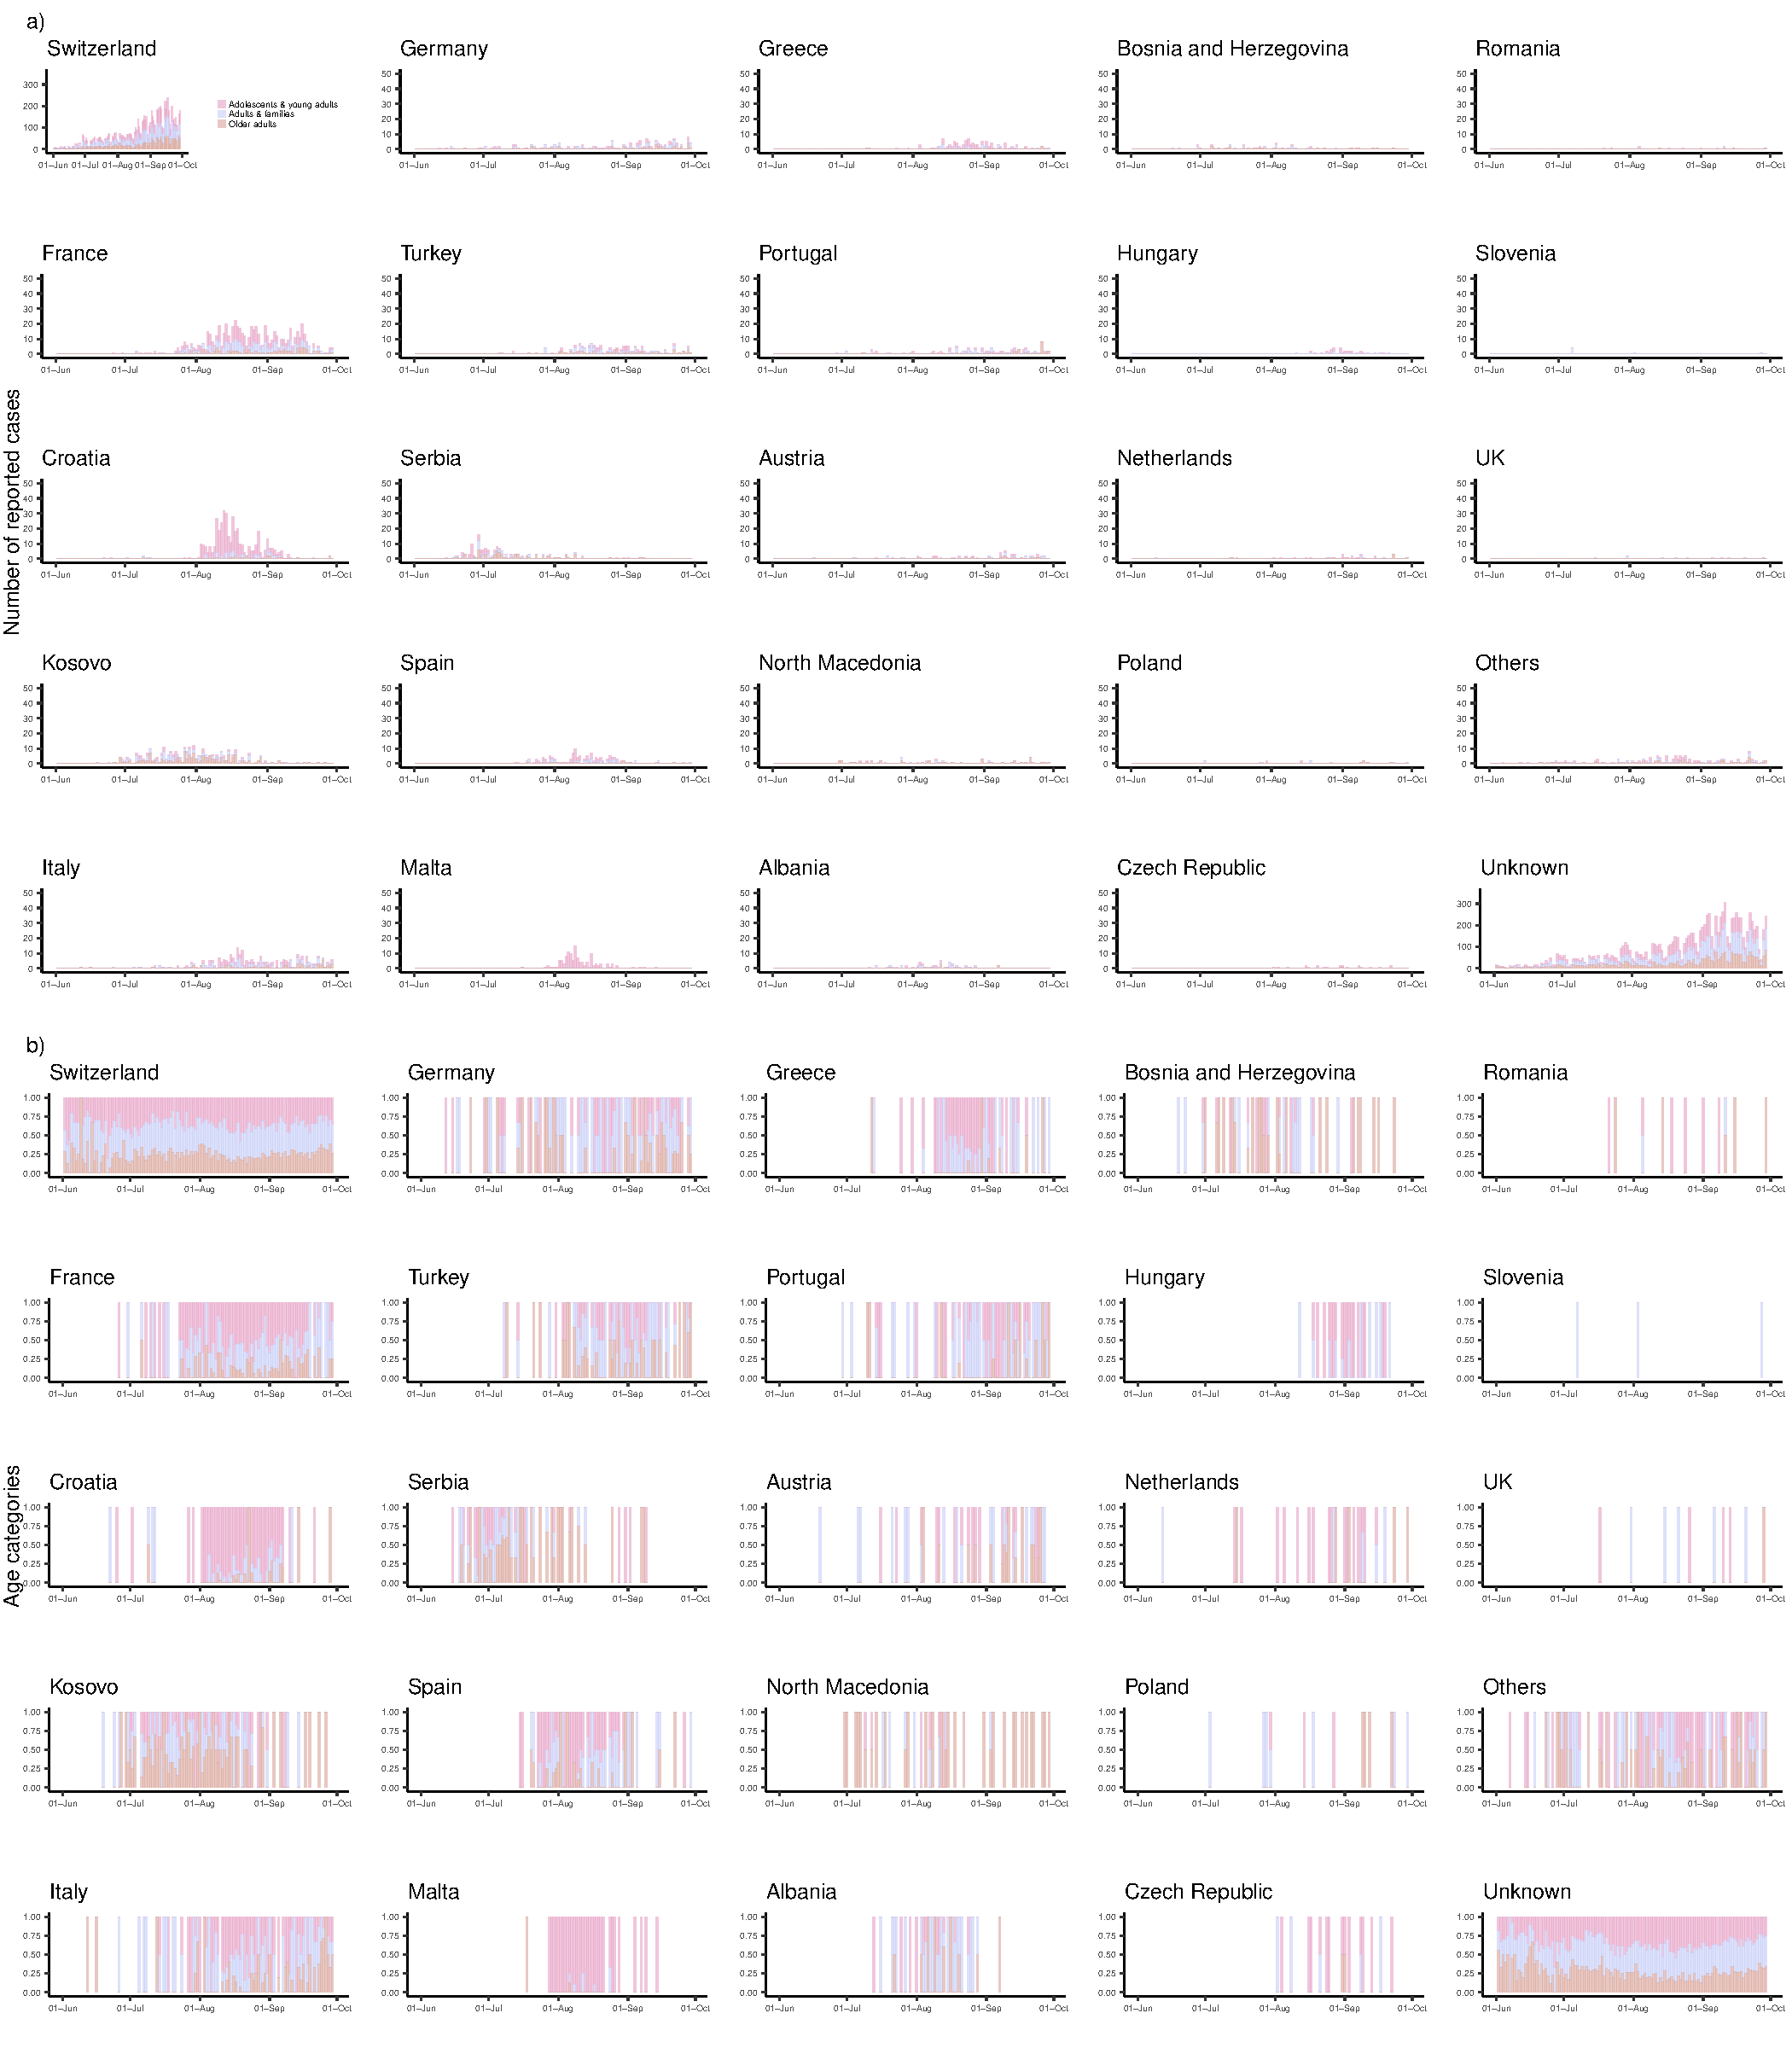
\includegraphics[scale=0.4]{imports_per_country_day_2021-03-05.pdf}
\caption{Reported cases and the most likely place of infection. a) y-axis and x-axis shows time of interest and number of reported cases b) y-axis and x-axis shows time of interest and proportion cases by different categories, i.e., adolescents and young adults (16-30 years), adults and families (31-50 and children up to 15 years), and older adults ($>$50 years).}
\end{suppfigure}
\clearpage
\begin{suppfigure}[h]
\centering
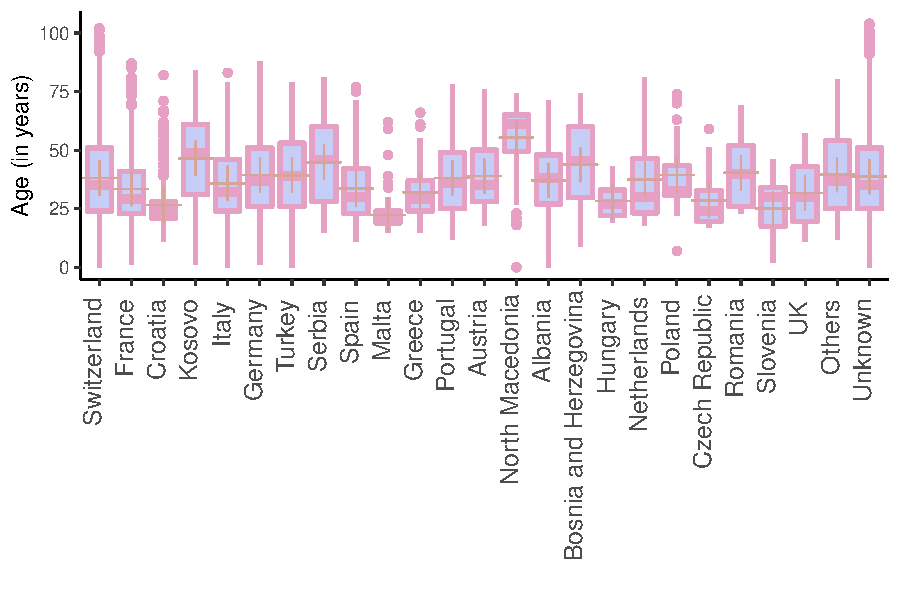
\includegraphics[scale=0.4]{age_percountry_2021-03-05.pdf}
\caption{Age distribution for reported cases by the most likely place of infection. y-axis and x-axis shows age and most likely infection place; + represents the mean.}
\end{suppfigure}

\begin{suppfigure}[h]
\centering
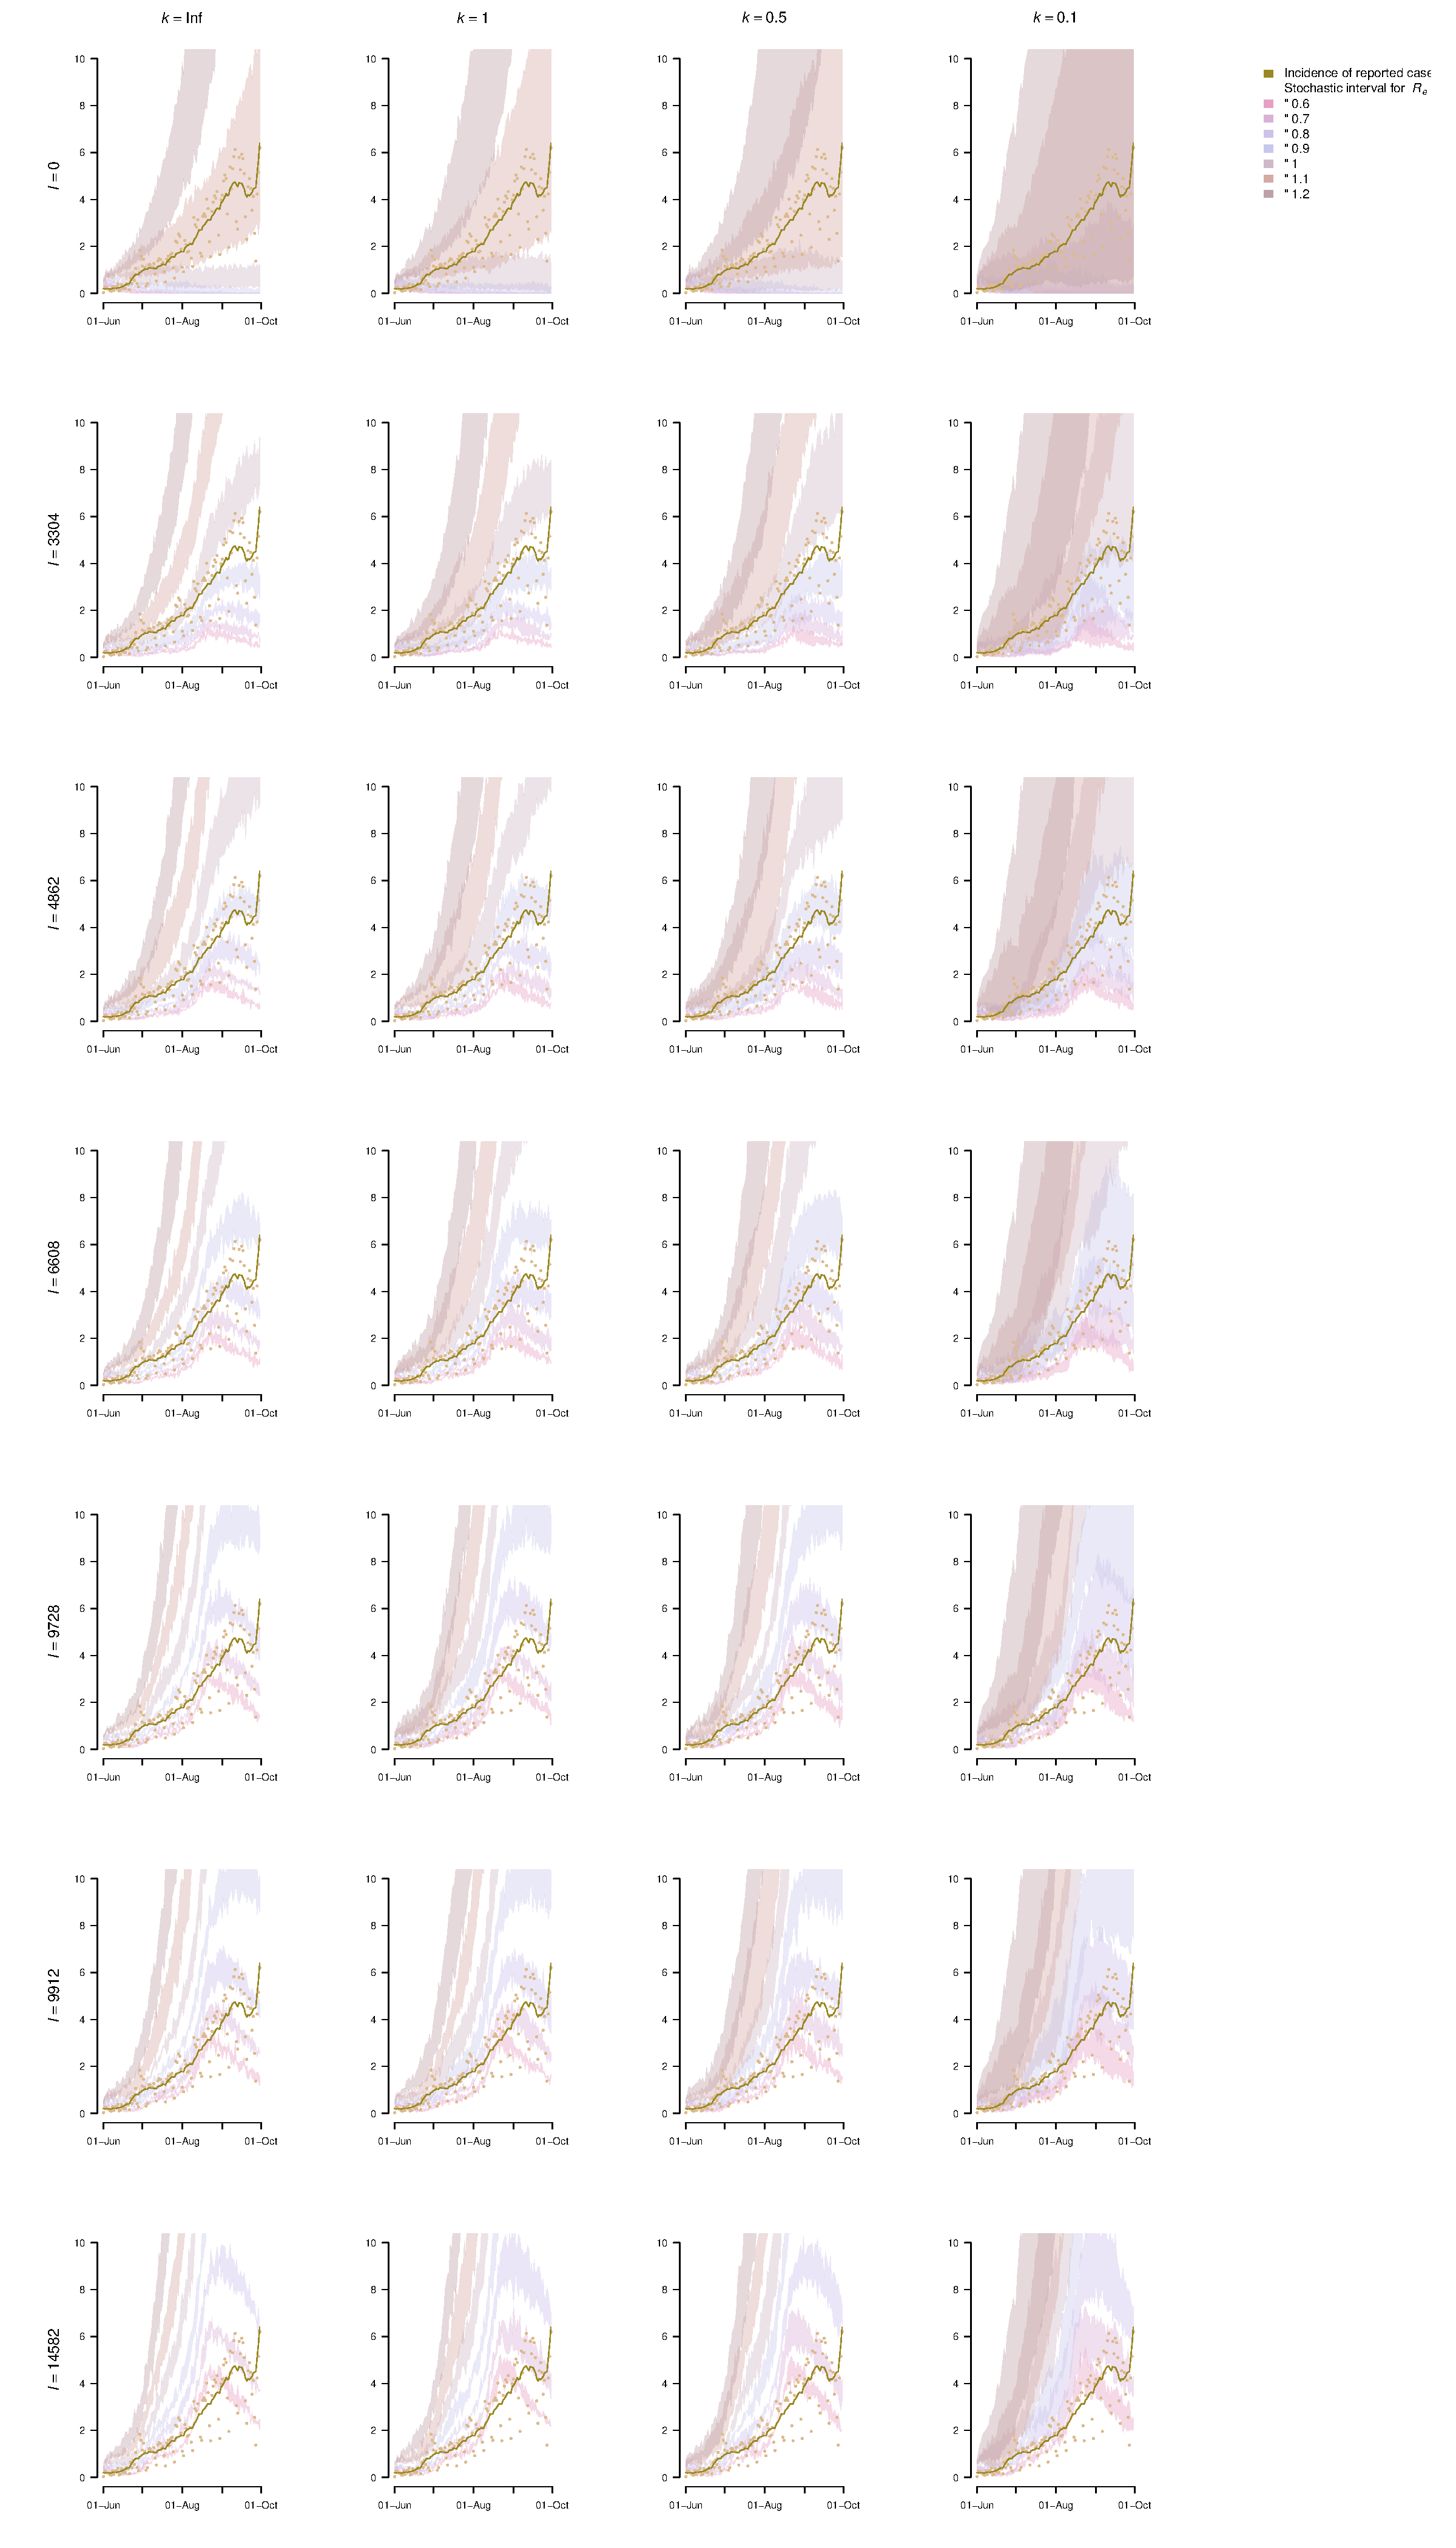
\includegraphics[scale=0.4]{incidence_sim_imports_infect_2021-03-10.pdf}
\caption{Incidence per day. y-axis incidence per 100,000; x-axis the time of interest. Green line represents weighted (mean of one week before and after) incidence of reported cases. Different number of travel-associated cases \emph{I} were added to a stochastic branching model whereby these \emph{I} could transmit further: \emph{I} was zero, reported \emph{I}, reported \emph{I} multiplied by $1+ \frac{\Sigma ~of ~cases ~with ~unknown ~origin }{\Sigma ~of ~all ~confirmed ~cases}$, and these multiplied with 2 and 3, respectively. Yellow dots show the reported cases per day and green area shows the predicted cases per day. Abbreviations: k, dispersion parameter; I, number of travel associated cases.}
\end{suppfigure}


\end{document}